
\chapter{Instalación}

Comenzamos instalando la máquina virtual como las anteriores, rellenando los datos relativos a la m3, como se muestra en \eqref{instal_1}.

\begin{figure}[h!]
\begin{center}
\caption{Instalación de m3}
\label{instal_1}
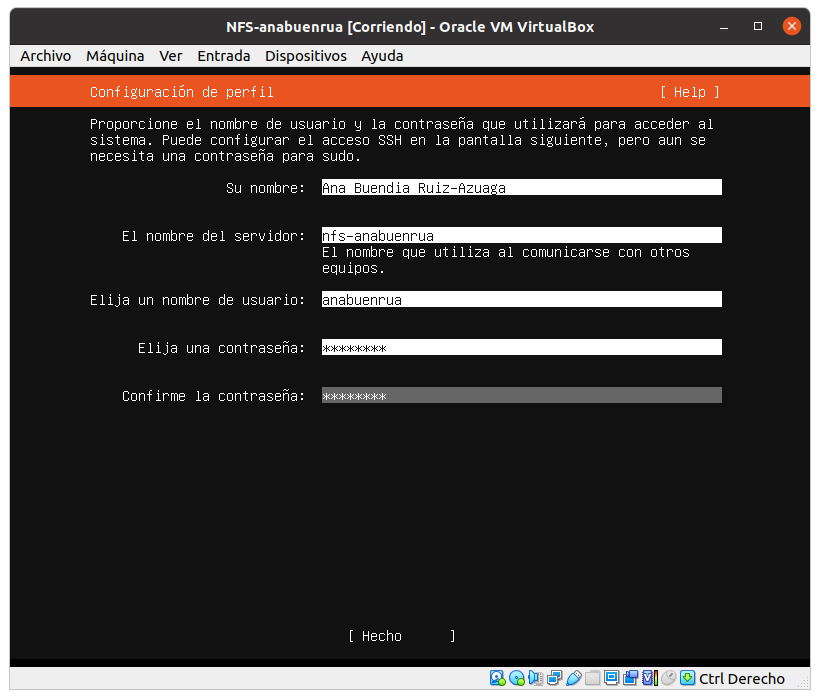
\includegraphics[scale=0.5]{instal_1}
\end{center}
\end{figure}

Añadimos el adaptador de red solo-anfitrión y configuramos la red editando el fichero \verb|/etc/netplan/00-installer-config.yaml| asignando la ip 192.168.56.103, \eqref{instal_3}.

\begin{figure}[h!]
\begin{center}
\caption{Configuración de la red de m3, fichero /etc/netplan/00-installer-config.yaml.}
\label{instal_3}
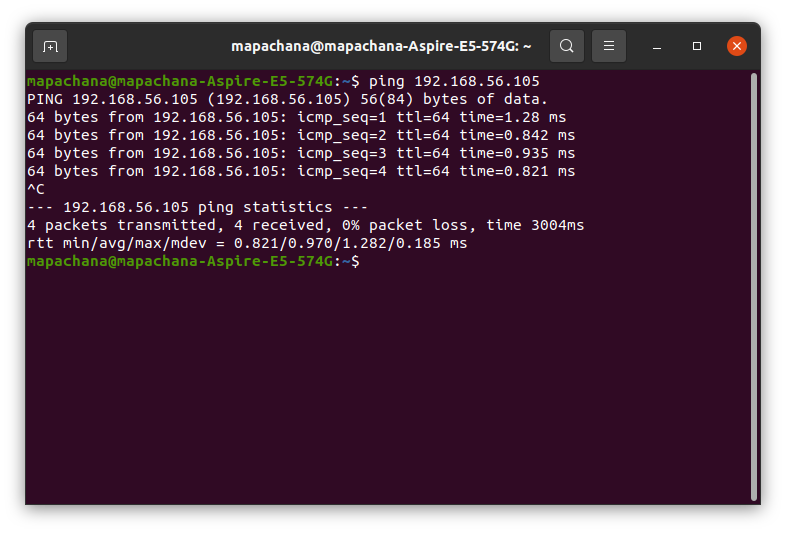
\includegraphics[scale=0.5]{instal_3}
\end{center}
\end{figure}

Finalmente ejecutamos \verb|sudo netplan apply| para hacer efectivos los cambios.

\chapter{Nginx}

Comenzamos instalando nginx, para ello ejecutamos:

\begin{verbatim}
sudo apt-get update && sudo apt-get dist-upgrade
&& sudo apt-get autoremove
sudo apt-get install nginx
\end{verbatim}

Lanzamos nginx con \verb|sudo systemctl start nginx|, y comprobamos que está activo, puede verse en \eqref{nginx_4}.

\begin{figure}[h!]
\begin{center}
\caption{Lanzamiento y comprobación del estado de nginx.}
\label{nginx_4}
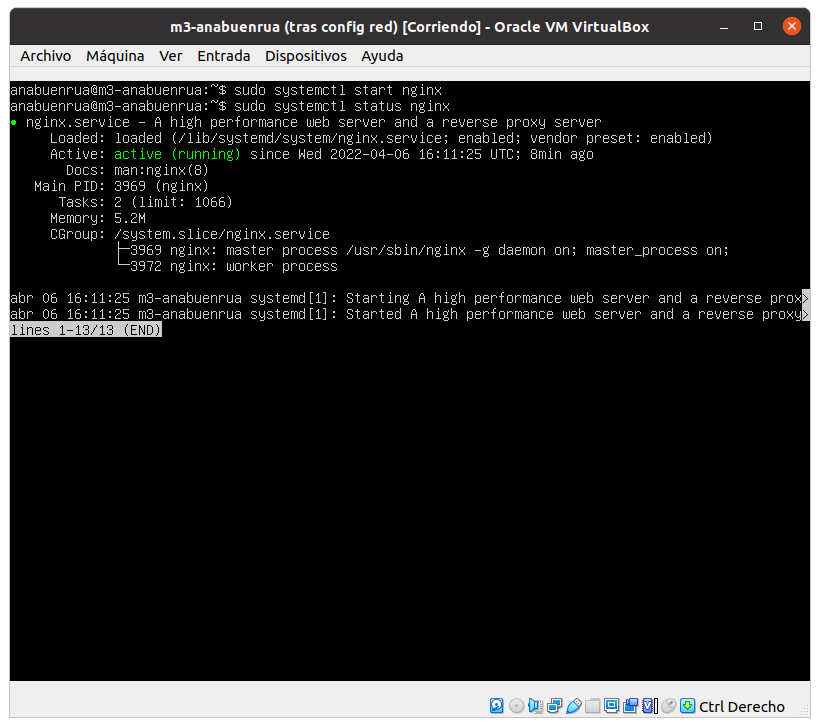
\includegraphics[scale=0.5]{nginx_4}
\end{center}
\end{figure}

Ahora deshabilitamos el servidor web para que nginx actúe como balanceador, para lo que vamos a editar el fichero \verb|/etc/nginx/nginx.conf|, dejándolo como en \eqref{nginx_5}:

\begin{figure}[h!]
\begin{center}
\caption{Deshabilitamos el servidor web modificando el fichero de configuración /etc/nginx/nginx.conf.}
\label{nginx_5}
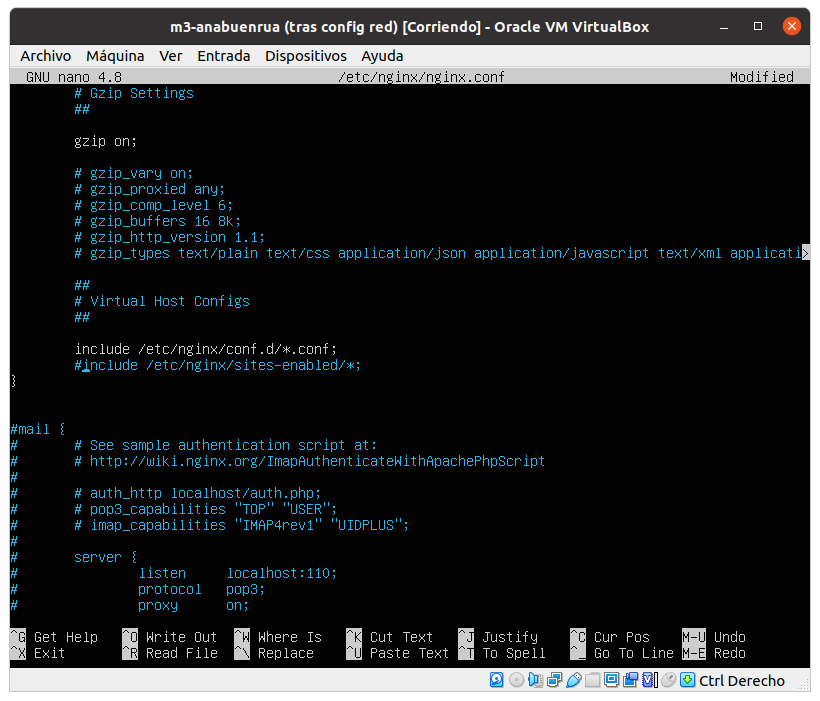
\includegraphics[scale=0.5]{nginx_5}
\end{center}
\end{figure}

Y ahora modificamos el archivo \verb|/etc/nginx/conf.d/default.conf| como se ve en \eqref{nginx_6}.

\begin{figure}[h!]
\begin{center}
\caption{Fichero de configuración /etc/nginx/conf.d/default.conf .}
\label{nginx_6}
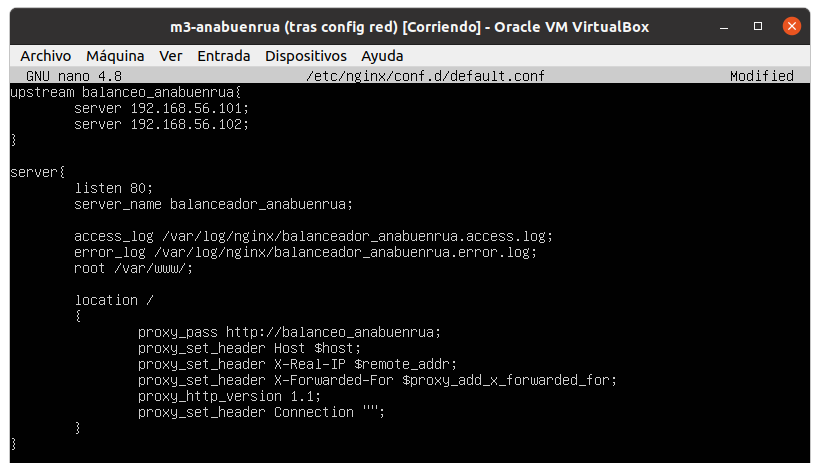
\includegraphics[scale=0.5]{nginx_6}
\end{center}
\end{figure}

Y reiniciamos el servicio con \verb|sudo systemctl restart nginx| para asegurarnos de que se aplica la configuración.

Comprobamos ahora accediendo a \verb|http://192.168.56.103/swap.html| en el navegador o mediante curl (como en \eqref{nginx_9}) que las máquinas se turnan para servir el sitio web.

\begin{figure}[h!]
\begin{center}
\caption{Comprobación del funcionamiento de la configuración de nginx con roundrobin.}
\label{nginx_9}
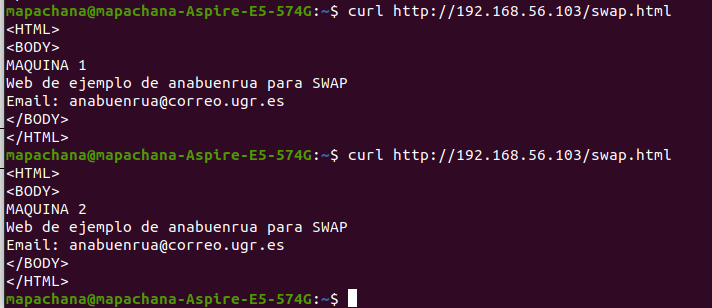
\includegraphics[scale=0.5]{nginx_9}
\end{center}
\end{figure}

\section{Ponderación}

Ahora vamos a repartir la carga entre las máquinas en función de pesos. Para ello, en \verb|/etc/nginx/conf.d/default.conf| vamos a usar el parámetro \verb|weight|.

Como ejemplo, vamos a suponer que m1 tiene el doble de capacidad que m2.

Editamos el fichero \verb|/etc/nginx/conf.d/default.conf| como en \eqref{nginx_10}.

\begin{figure}[h!]
\begin{center}
\caption{Fichero de configuración /etc/nginx/conf.d/default.conf para ponderación.}
\label{nginx_10}
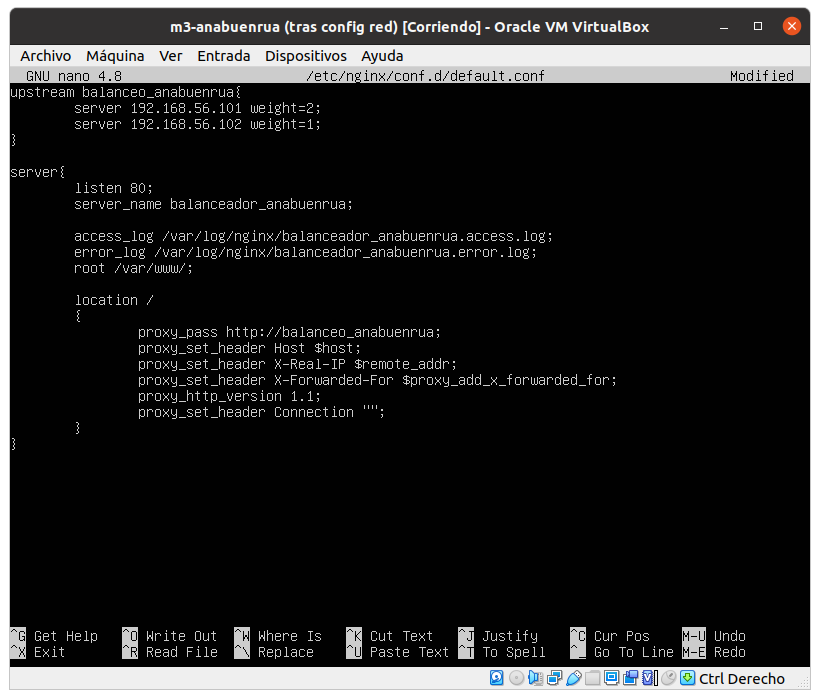
\includegraphics[scale=0.5]{nginx_10}
\end{center}
\end{figure}

Relanzamos nginx con \verb|sudo systemctl restart nginx| y comprobamos que funciona en \eqref{nginx_11}.

\begin{figure}[h!]
\begin{center}
\caption{Comprobación del funcionamiento de la configuración de nginx con ponderación.}
\label{nginx_11}
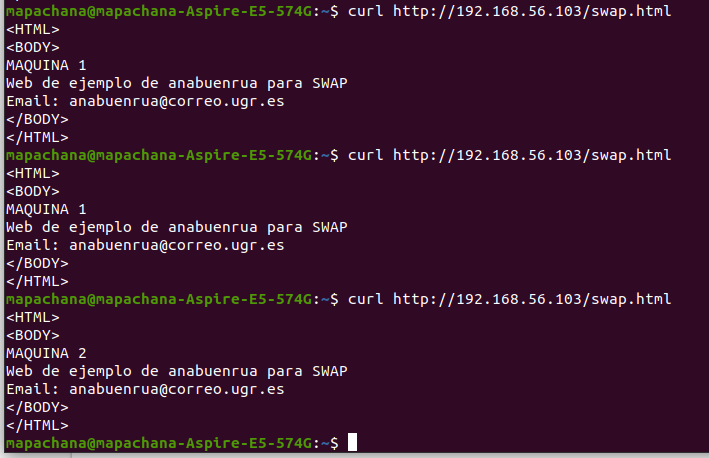
\includegraphics[scale=0.5]{nginx_11}
\end{center}
\end{figure}

\section{Otras opciones avanzadas}

Ahora vamos a configurar que todas las peticiones que vengan de la misma IP se dirijan a la misma máquina servidora final. Para ello, usamos \verb|ip_hash| en el fichero de configuración, como en \eqref{nginx_12}.

\begin{figure}[h!]
\begin{center}
\caption{Fichero de configuración /etc/nginx/conf.d/default.conf con ip\_hash.}
\label{nginx_12}
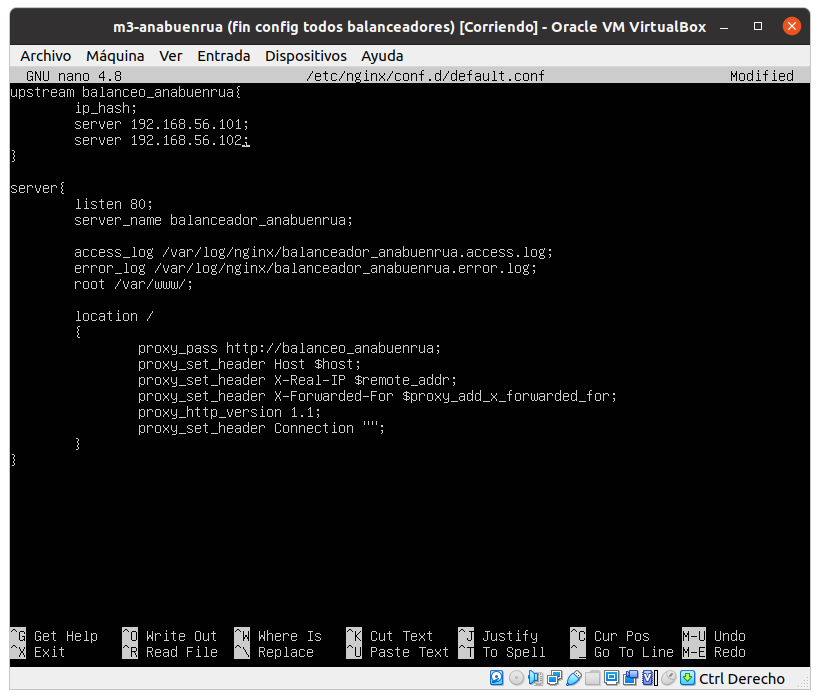
\includegraphics[scale=0.5]{nginx_12a}
\end{center}
\end{figure}

De nuevo, reiniciamos el servicio para hacer efectiva la configuración y comprobamos que funciona en \eqref{nginx_13}.

\begin{figure}[h!]
\begin{center}
\caption{Comprobación del funcionamiento de la configuración de nginx con ip\_hash.}
\label{nginx_13}
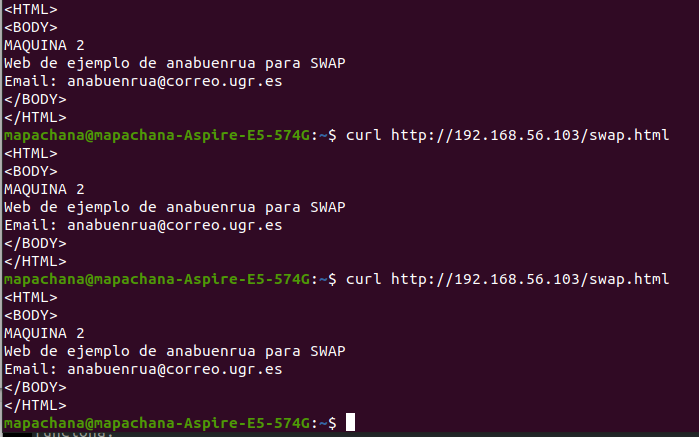
\includegraphics[scale=0.5]{nginx_13}
\end{center}
\end{figure}

También podemos activar las conexiones \verb|keepalive| por 3 segundos, ilustrado en \eqref{nginx_14}.

\begin{figure}[h!]
\begin{center}
\caption{Fichero de configuración /etc/nginx/conf.d/default.conf con keepalive.}
\label{nginx_14}
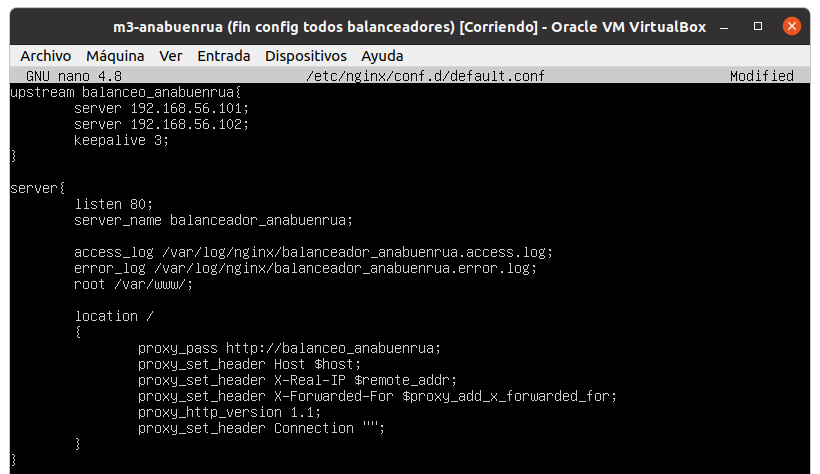
\includegraphics[scale=0.5]{nginx_14a}
\end{center}
\end{figure}

Otra opción es usar \verb|down|, que marca un servidor como permanentemente offline, y requiere de ser usado con \verb|ip_hash|, como se ve en \eqref{nginx_15}.

\begin{figure}[h!]
\begin{center}
\caption{Fichero de configuración /etc/nginx/conf.d/default.conf con down.}
\label{nginx_15}
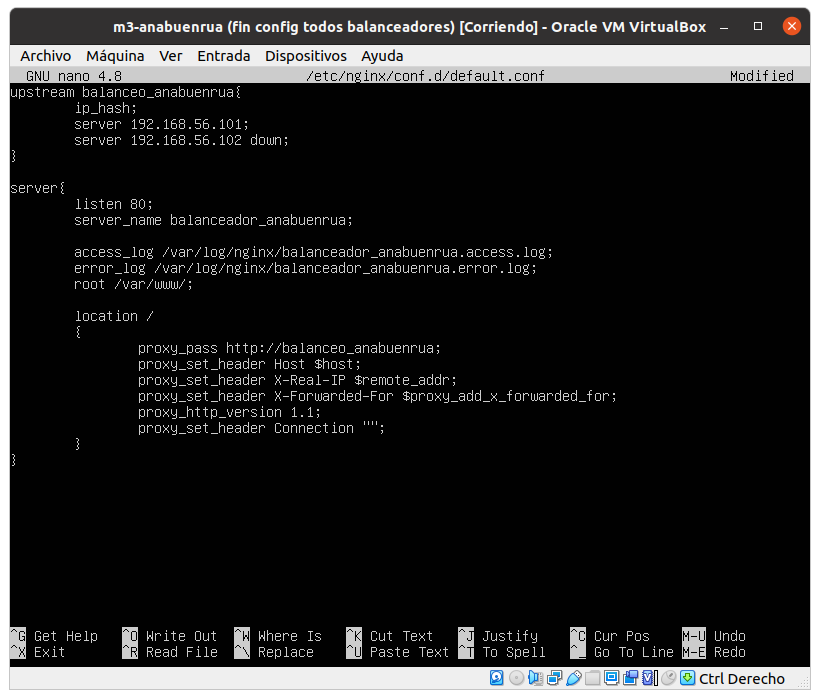
\includegraphics[scale=0.5]{nginx_15a}
\end{center}
\end{figure}

Relanzamos el servicio y comprobamos que funciona en \eqref{nginx_16}.

\begin{figure}[h!]
\begin{center}
\caption{Comprobación del funcionamiento de la configuración de nginx con down.}
\label{nginx_16}
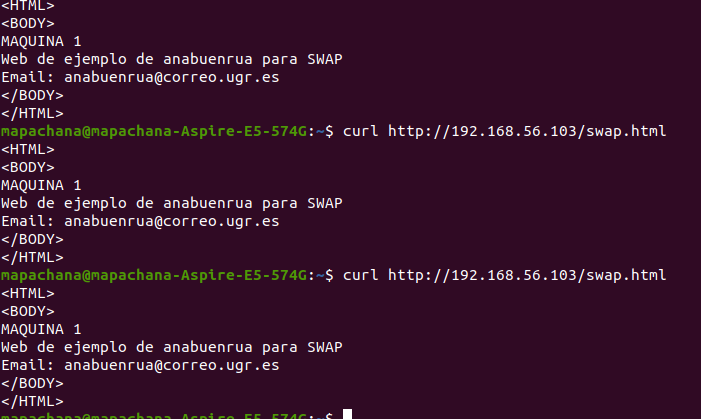
\includegraphics[scale=0.5]{nginx_16}
\end{center}
\end{figure}

También podemos usar \verb|backup|, que reserva este servidor y solo le pasa tráfico si alguno de los otros servidores no configurados como backup está caído u ocupado, como se muestra en \eqref{nginx_17}.

\begin{figure}[h!]
\begin{center}
\caption{Fichero de configuración /etc/nginx/conf.d/default.conf con backup.}
\label{nginx_17}
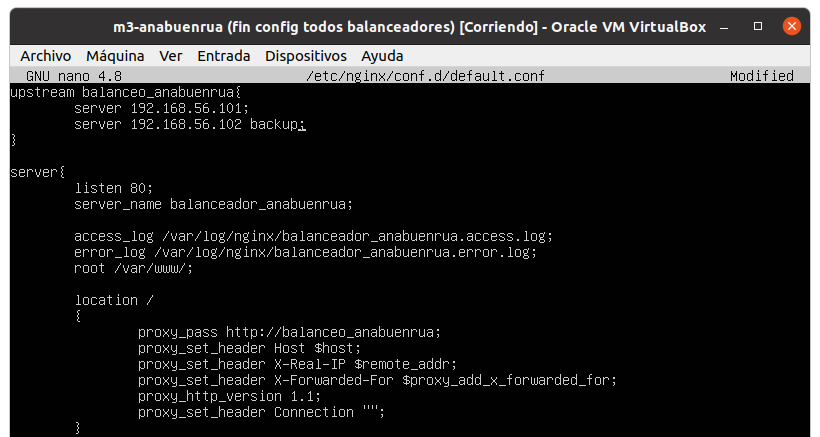
\includegraphics[scale=0.5]{nginx_17a}
\end{center}
\end{figure}

Y ahora siempre nos atiende m1.

Finalmente, para evitar errores al reiniciar la máquina virtual, se va a deshabilitar que se lance nginx al encender la máquina. Para ello se ejecuta \verb|sudo systemctl disable nginx|.

\chapter{HAProxy}

Comenzamos parando nginx, de forma que no interfiera con HAProxy, ya que usan el mismo puerto. Para pararlo, ejecutamos \verb|sudo systemctl stop nginx|.

Ahora instalamos HAproxy con \verb|sudo apt-get install haproxy|.

Lanzamos HAProxy con \verb|sudo systemctl start haproxy| y comprobamos su estado, como se muestra en \eqref{haproxy_2}.

\begin{figure}[h!]
\begin{center}
\caption{Lanzamiento y comprobación del estado de haproxy.}
\label{haproxy_2}
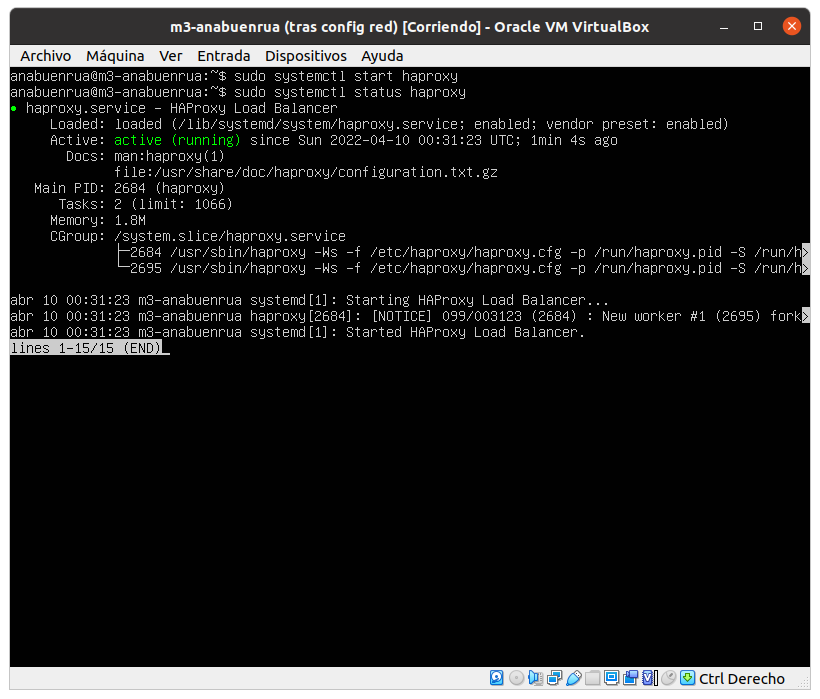
\includegraphics[scale=0.5]{haproxy_2}
\end{center}
\end{figure}

Editamos ahora el archivo de configuración \verb|/etc/haproxy/haproxy.cfg| como en \eqref{haproxy_3}.

\begin{figure}[h!]
\begin{center}
\caption{Fichero de configuración /etc/haproxy/haproxy.cfg .}
\label{haproxy_3}
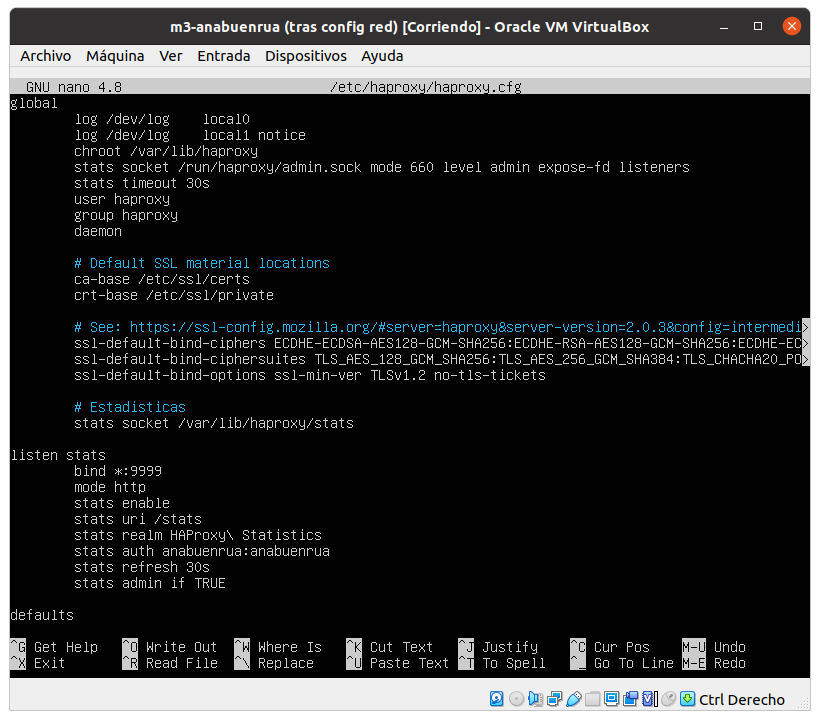
\includegraphics[scale=0.5]{haproxy_4}
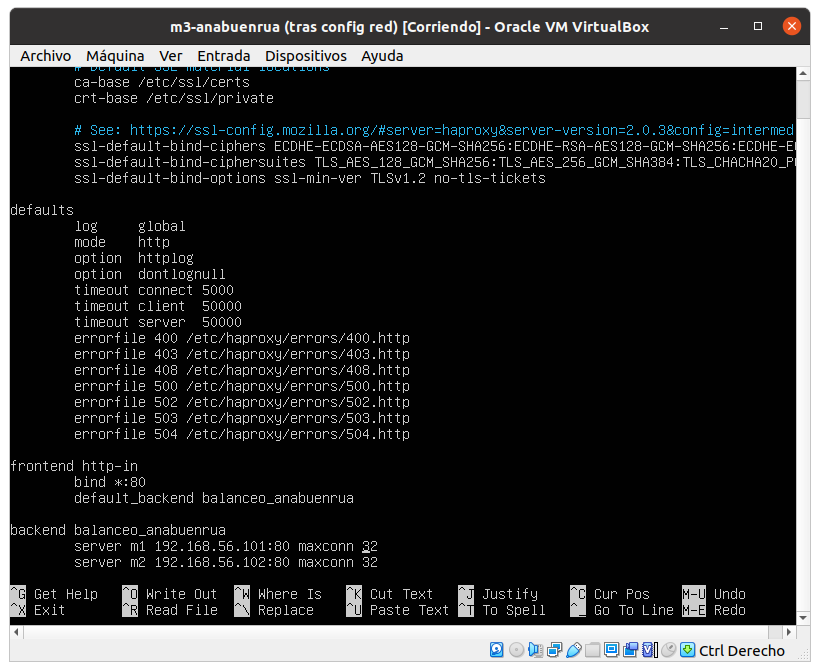
\includegraphics[scale=0.5]{haproxy_3}
\end{center}
\end{figure}

Y relanzamos el servicio con \verb|sudo systemctl restart haproxy|.

Comprobamos que funciona, va sirviendo por turnos cada máquina, al igual que lo hacía nginx.

\section{Ponderación}

Para configurar la ponderación, de nuevo editamos el fichero \verb|/etc/haproxy/haproxy.cfg|, usando la opción weight. De nuevo se ha supuesto a m1 con el doble de capacidad de m2, como se ve en \eqref{haproxy_5}.

\begin{figure}[h!]
\begin{center}
\caption{Fichero de configuración /etc/haproxy/haproxy.cfg para ponderación.}
\label{haproxy_5}
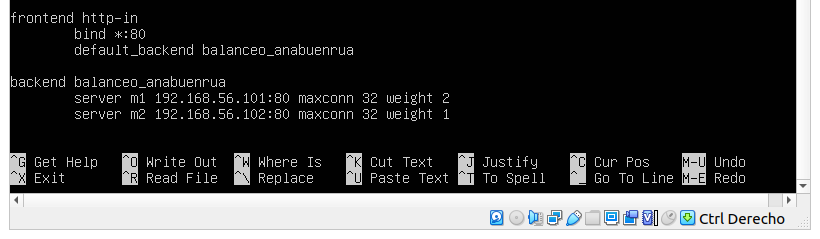
\includegraphics[scale=0.5]{haproxy_5}
\end{center}
\end{figure}

Y relanzamos el servicio y comprobamos que funciona, de nuevo m1 sirve 2 de cada 3 peticiones que realizamos.

\section{Opciones avanzadas}

Por analogía y para que sirva de comparativa con cómo se realizan algunas configuraciones en nginx, se van a usar configuraciones ya usadas antes.

Por ejemplo, para usar ip hash, editando de nuevo el archivo de configuración como en \eqref{haproxy_7}.

\begin{figure}[h!]
\begin{center}
\caption{Fichero de configuración /etc/haproxy/haproxy.cfg para ip\_hash.}
\label{haproxy_7}
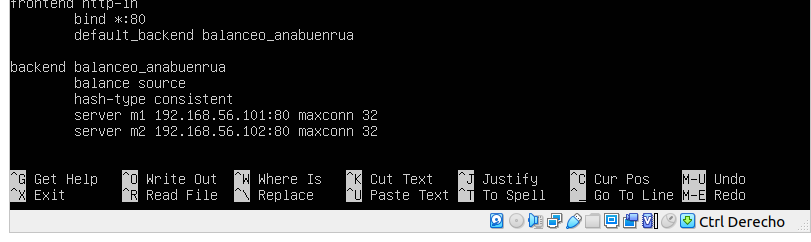
\includegraphics[scale=0.5]{haproxy_7a}
\end{center}
\end{figure}

Y relanzamos y comprobamos que funciona, pues siempre nos atiende m1.

Además, también podemos poner de nuevo m2 en backup, como se muestra en \eqref{haproxy_9}.

\begin{figure}[h!]
\begin{center}
\caption{Fichero de configuración /etc/haproxy/haproxy.cfg con backup.}
\label{haproxy_9}
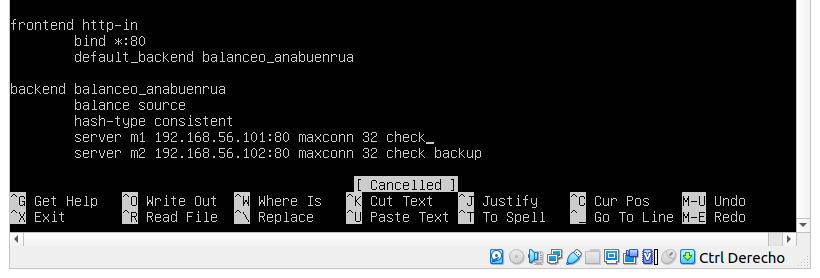
\includegraphics[scale=0.5]{haproxy_9}
\end{center}
\end{figure}

Y relanzando comprobamos que funciona, ya que siempre nos atiende m1.

Finalmente, para evitar errores al reiniciar la máquina virtual, se va a deshabilitar que se lance HAProxy al encender la máquina. Para ello se ejecuta \verb|sudo systemctl disable haproxy|.

\chapter{Estadísticas de HAProxy}

Para esta sección dejamos round-robin, como en la configuración inicial, y añadimos configuración necesaria para habilitar las estadísticas en \verb|/etc/haproxy/haproxy.cfg|, como se ve en \eqref{estad_1}.

\begin{figure}[h!]
\begin{center}
\caption{Fichero de configuración /etc/haproxy/haproxy.cfg para habilitar estadísicas.}
\label{estad_1}
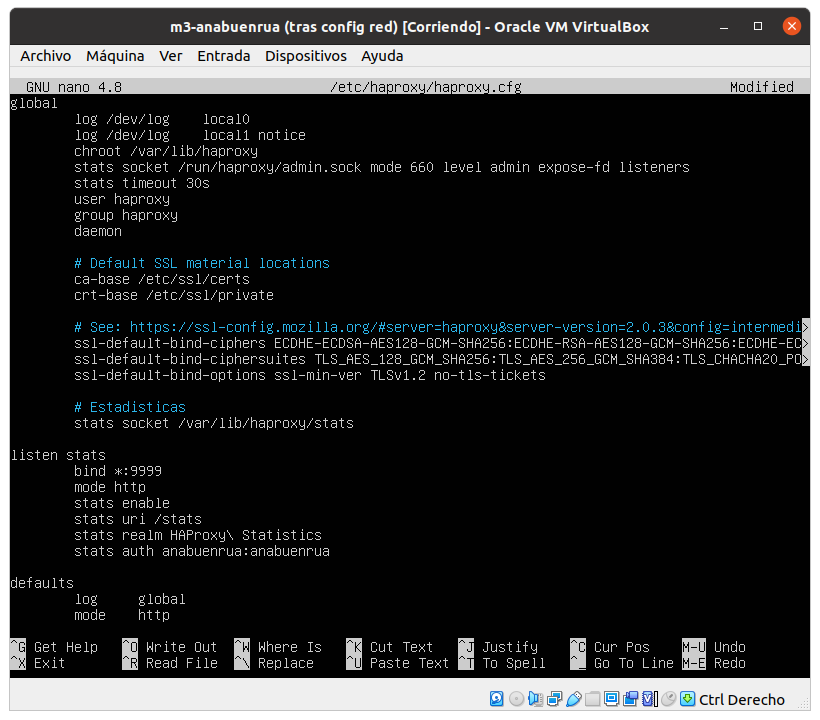
\includegraphics[scale=0.5]{estad_1}
\end{center}
\end{figure}

Relanzamos haproxy y accedemos a las estadísticas, para lo que introducimos el usuario y contraseña antes de acceder, como puede verse en \eqref{estad_2}.

\begin{figure}[h!]
\begin{center}
\caption{Accediendo a las estadísticas de HAProxy a través del navegador}
\label{estad_2}
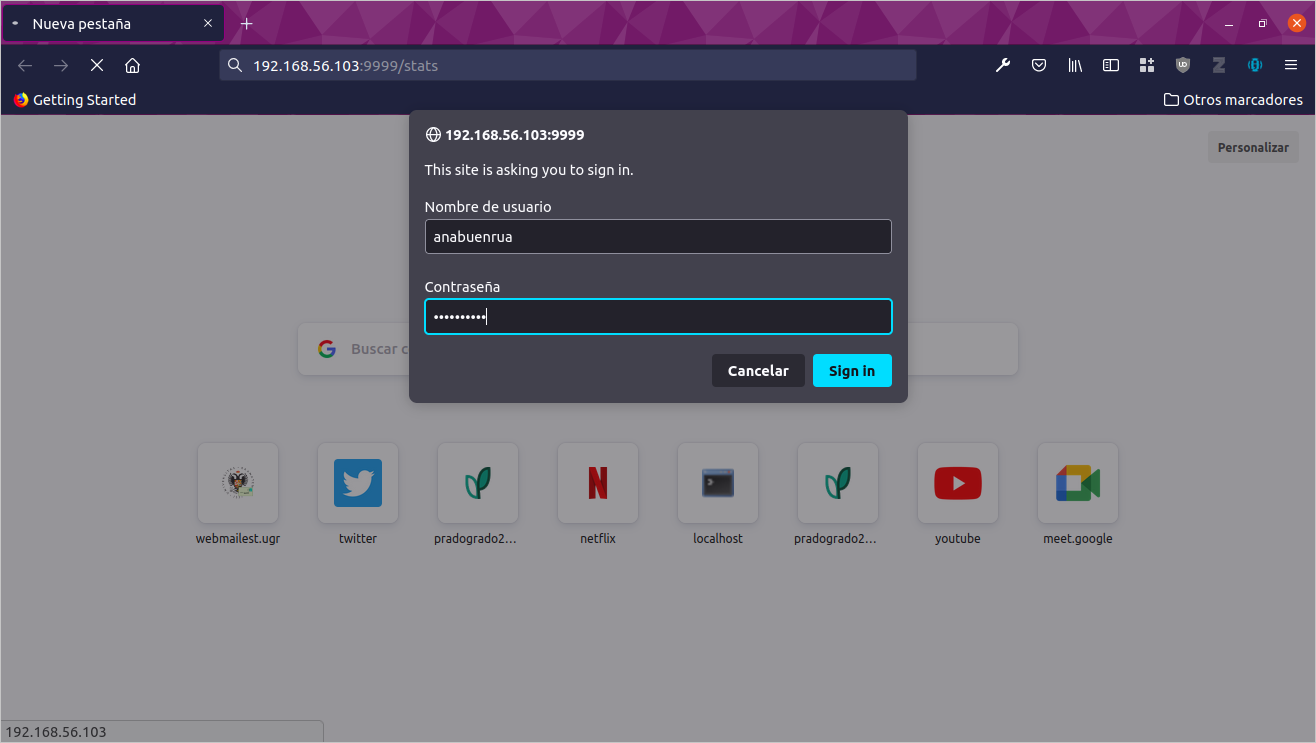
\includegraphics[scale=0.5]{estad_2}
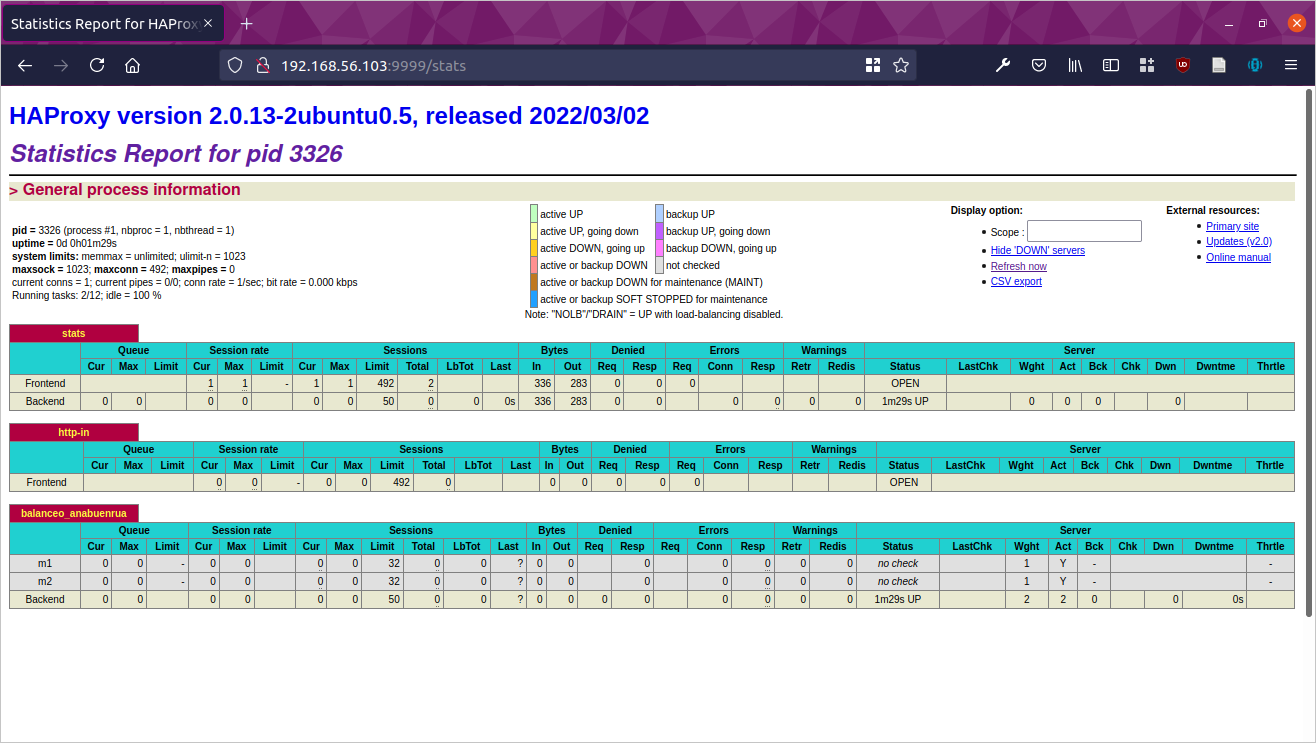
\includegraphics[scale=0.35]{estad_3}
\end{center}
\end{figure}

\section{Opciones avanzadas}

Como opciones avanzadas se va a añadir el tiempo de refresco de la página y la posibilidad de marcar los servidores como down o maintenance.

Por ejemplo, vamos a usar un tiempo de refresco de 30 segundos.

Para ello, editamos de nuevo el fichero de configuración añadiendo las líneas:

\begin{verbatim}
stats refresh 30s
stats admin if TRUE
\end{verbatim}

Luego el fichero quedaría como \eqref{estad_4}.

\begin{figure}[h!]
\begin{center}
\caption{Fichero de configuración /etc/haproxy/haproxy.cfg con opciones avanzadas de las estadísticas.}
\label{estad_4}
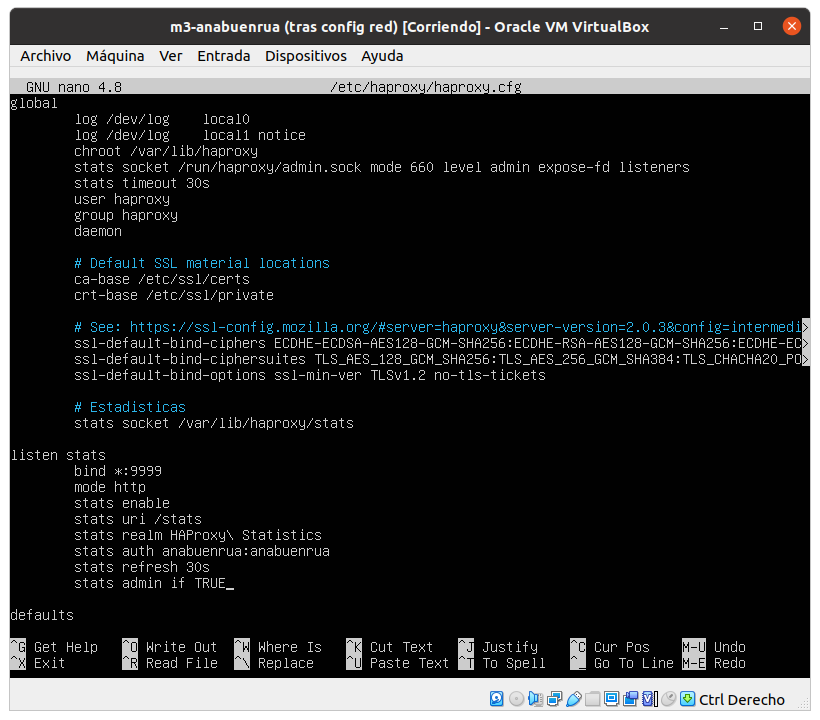
\includegraphics[scale=0.5]{estad_4}
\end{center}
\end{figure}

Y relanzando de nuevo el servicio y accediendo a las estadísticas observamos los cambios en \eqref{estad_5}.

\begin{figure}[h!]
\begin{center}
\caption{Estadísticas de haproxy con opciones avanzadas.}
\label{estad_5}
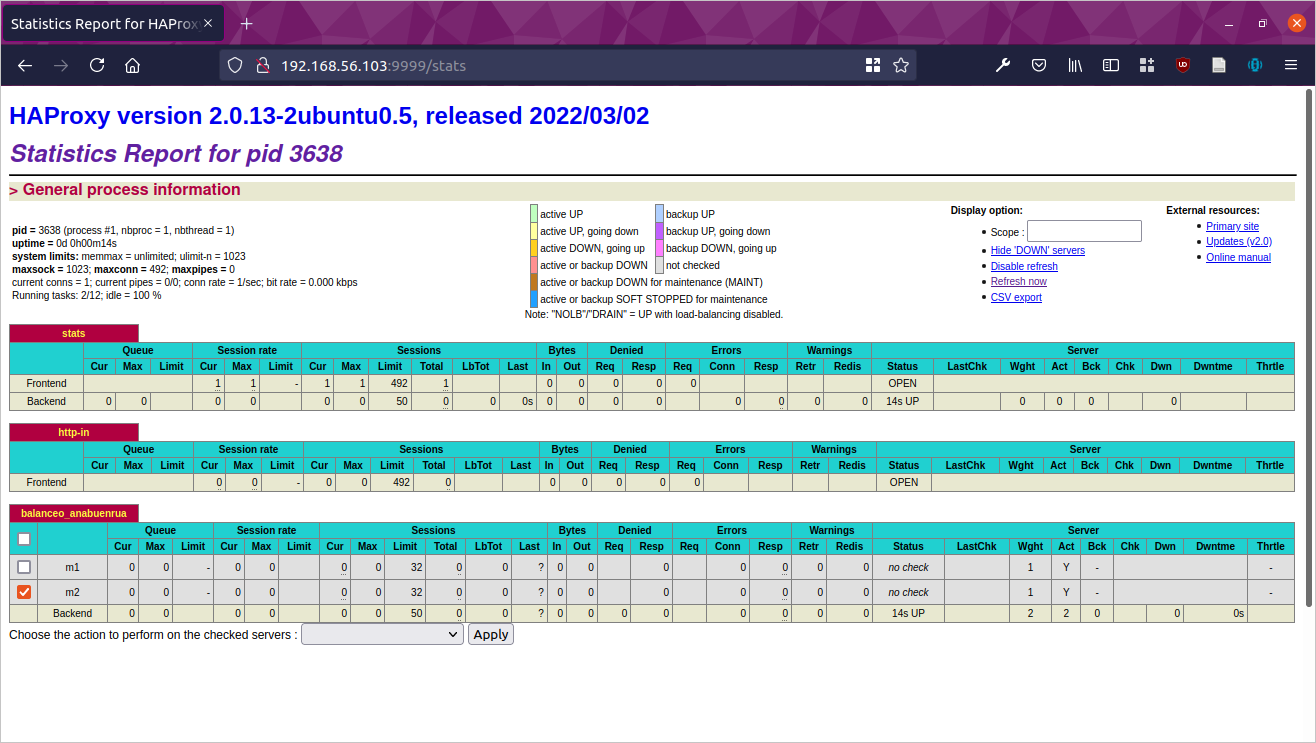
\includegraphics[scale=0.35]{estad_5}
\end{center}
\end{figure}

Si además se quisiera configurar el timeout, se usaría \verb|stats timeout <n>s|.

\chapter{Gobetween}

Comenzamos asegurándonos de que tanto nginx como haproxy no se estén ejecutando, y tras esto instalamos gobetween mediante snap ejecutando:

\begin{verbatim}
sudo snap install gobetween --edge
\end{verbatim}

Ahora, vamos a configurar gobetween, para ello nos basamos en el archivo de configuración de \verb|/snap/gobetween/current/config/gobetween.toml|, y creamos el fichero de configuración \verb|/snap/gobetween/gobetween_config.toml| quedando como \eqref{gobet_3}.

\begin{figure}[h!]
\begin{center}
\caption{Fichero de configuración /snap/gobetween/gobetween\_config.toml }
\label{gobet_3}
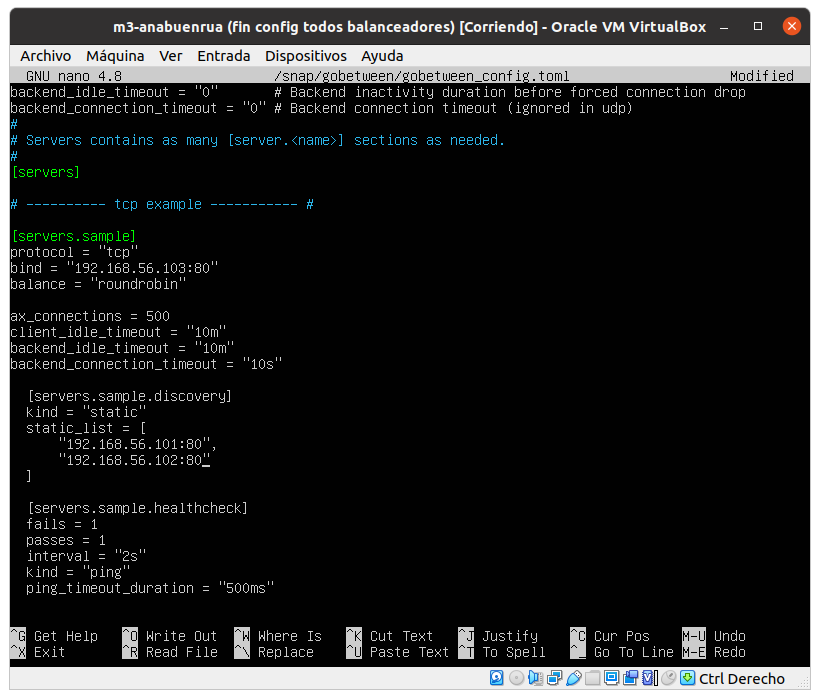
\includegraphics[scale=0.5]{gobet_3a}
\end{center}
\end{figure}

Hemos dejado los parámetros por defecto que venían (defaults) y las métricas activadas, ya que esta configuración ya venía realizada en la configuración de ejemplo. Las opciones de healthcheck se explicarán en el apartado de opciones avanzadas.

Y ahora lanzamos gobetween con la configuración establecida indicando el fichero. Como vemos en \eqref{gobet_4}, no tenemos permiso de escucha para el puerto 80, y nos lanza un error.

\begin{figure}[h!]
\begin{center}
\caption{Error al lanzar gobetween por no tener permisos de escucha del puerto 80.}
\label{gobet_4}
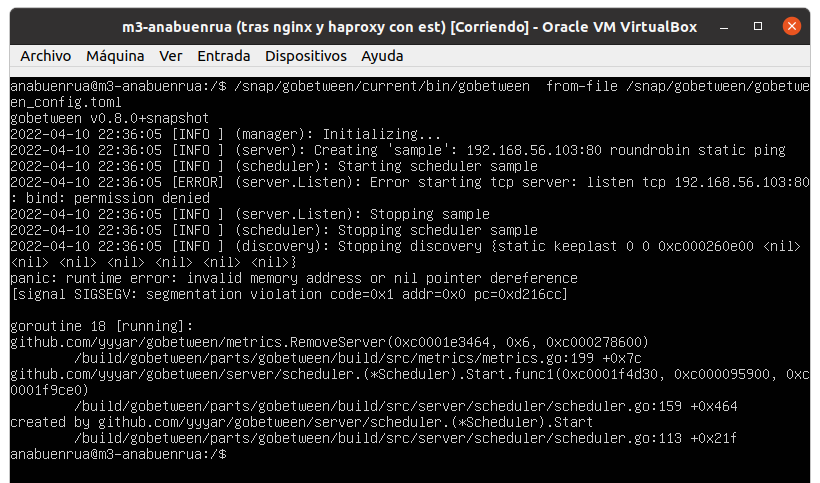
\includegraphics[scale=0.5]{gobet_4}
\end{center}
\end{figure}

Por tanto, ejecutamos gobetween con sudo, de forma que no da problemas, como puede verse en \eqref{gobet_5}.

\begin{figure}[h!]
\begin{center}
\caption{Lanzamiento de gobetween con sudo.}
\label{gobet_5}
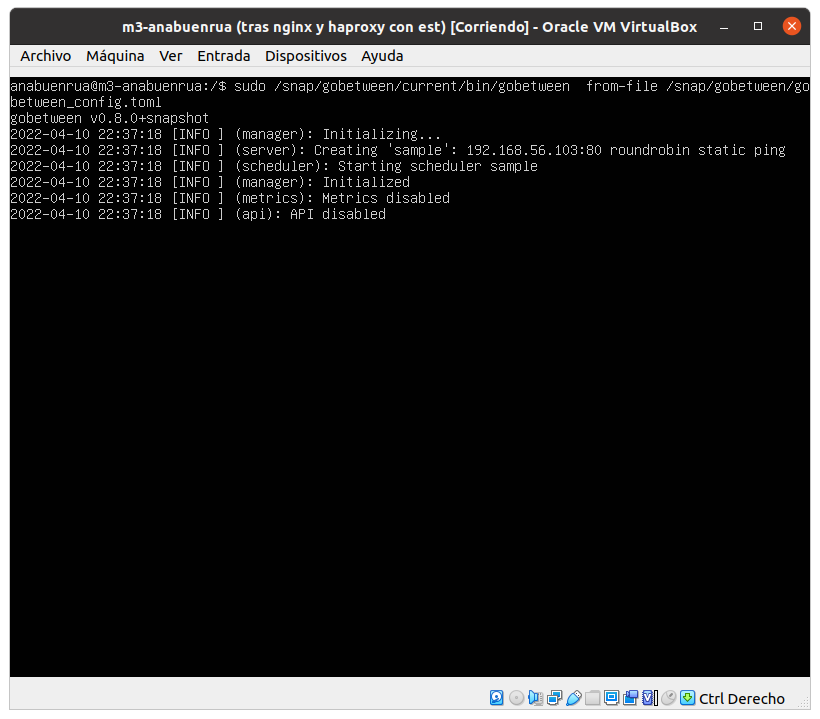
\includegraphics[scale=0.5]{gobet_5}
\end{center}
\end{figure}

Y comprobamos que funciona, pues las máquinas m1 y m2 responden turnándose.

\section{Opciones avanzadas}

Además de round-robin, se puede usar ip\_hash como se muestra en \eqref{gobet_7}, también menor número de conexiones \eqref{gobet_8} y por ponderación \eqref{gobet_9}.

\begin{figure}[h!]
\begin{center}
\caption{Fichero de configuración /snap/gobetween/gobetween\_config.toml con ip\_hash}
\label{gobet_7}
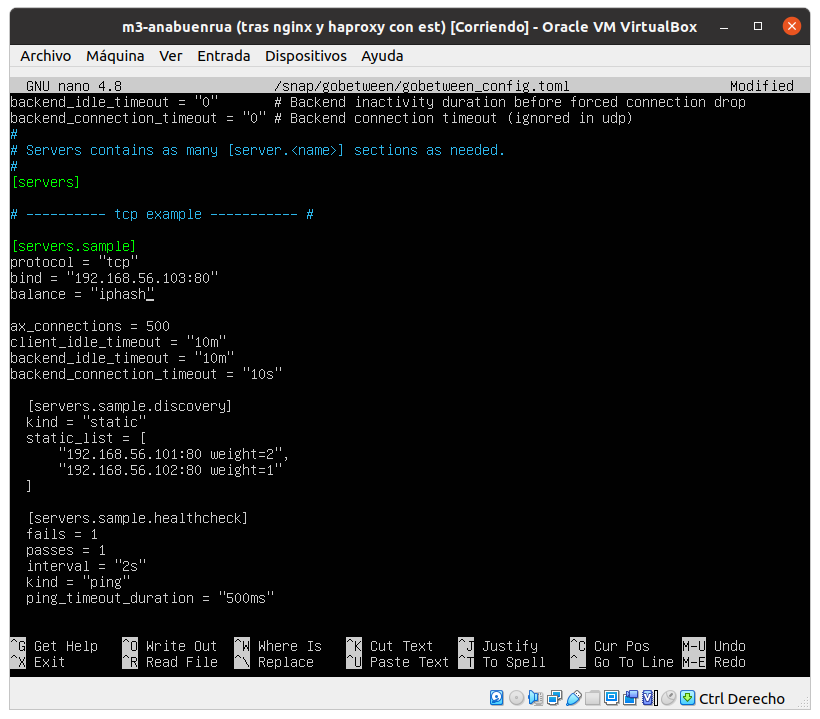
\includegraphics[scale=0.5]{gobet_7}
\end{center}
\end{figure}

\begin{figure}[h!]
\begin{center}
\caption{Fichero de configuración /snap/gobetween/gobetween\_config.toml con mínimo número de conexiones}
\label{gobet_8}
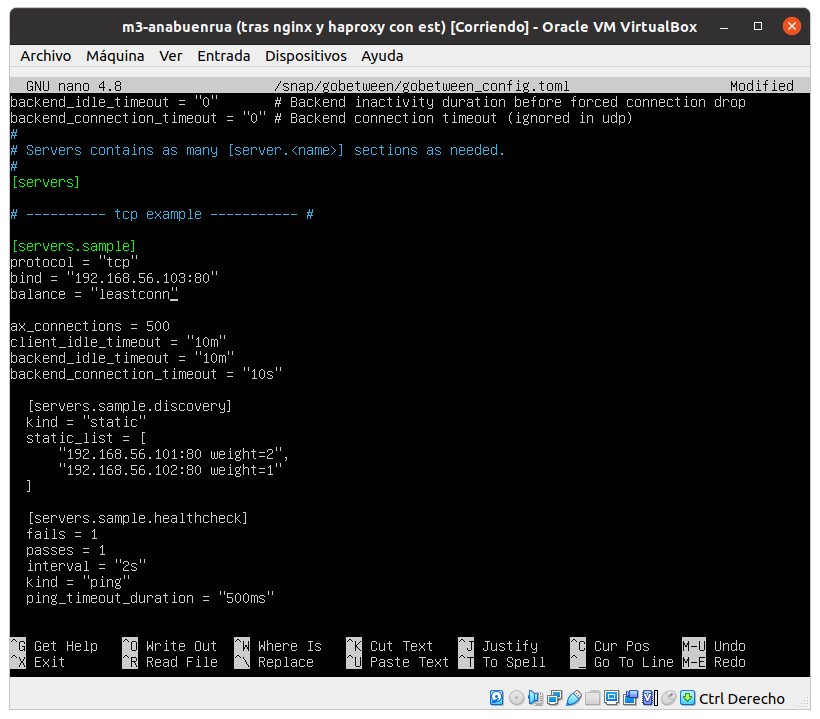
\includegraphics[scale=0.5]{gobet_8}
\end{center}
\end{figure}

\begin{figure}[h!]
\begin{center}
\caption{Fichero de configuración /snap/gobetween/gobetween\_config.toml con ponderación}
\label{gobet_9}
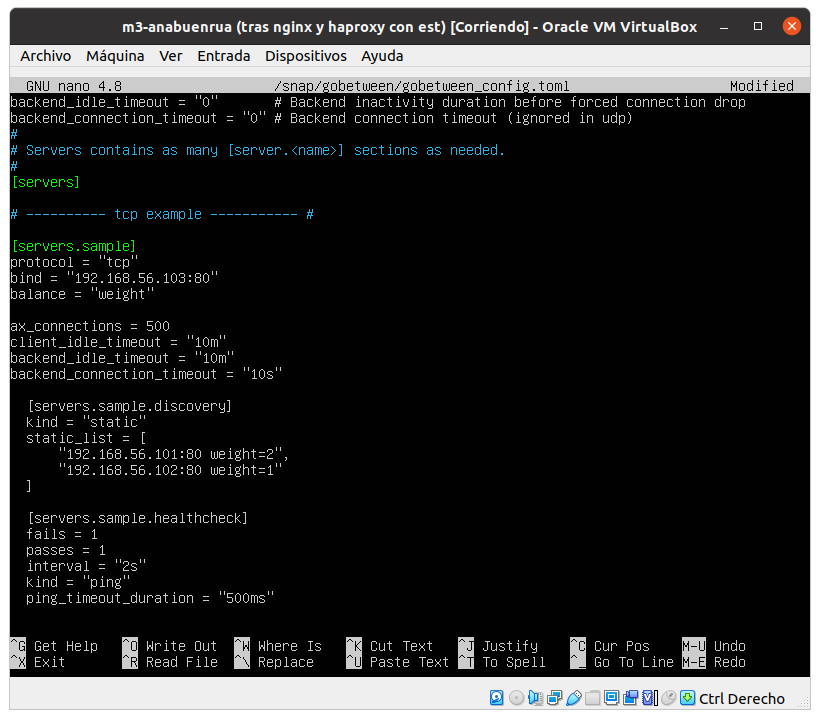
\includegraphics[scale=0.5]{gobet_9}
\end{center}
\end{figure}

Adicionalmente, se ha configurado el último bloque, \verb|healthcheck|, que comprueba el estado de los servidores mediante ping (pues se ha configurado con este método) cada 2 segundos, y debe llegar una respuesta antes de 500ms. Si esta respuesta no llegara, como se ha perdido una respuesta (parámetro fails está a 1), el servidor se considera caído (down), y se marcará de nuevo como operativo cuando llegue una respuesta de un ping (parámetro passes está a 1).

En este caso, como gobetween no es un servicio, no hace falta desactivar que se lance automáticamente al encender la máquina virtual.

\chapter{Zevenet}

Para configurar Zevenet, vamos a instalar una iso, que descargamos de

\href{https://es.zevenet.com/productos/comunidad/}{https://es.zevenet.com/productos/comunidad/}.

Comenzamos creando una nueva máquina virtual, de nuevo con 1GB de RAM, 10GB de disco duro dinámico y añadimos el adaptador de red solo-anfitrión antes de iniciar la máquina, de modo que detecte tanto el adaptador NAT como el solo-anfitrión automáticamente.

Al instalarlo, lo hacemos en español de España seleccionando el teclado español, luego seleccionamos el segundo adaptador de red \eqref{zev_2} e introducimos la IP de la máquina \eqref{zev_3}, en este caso se ha usado 192.168.56.104.

\begin{figure}[h!]
\begin{center}
\caption{Selección del adaptador de red durante la instalación de Zevenet.}
\label{zev_2}
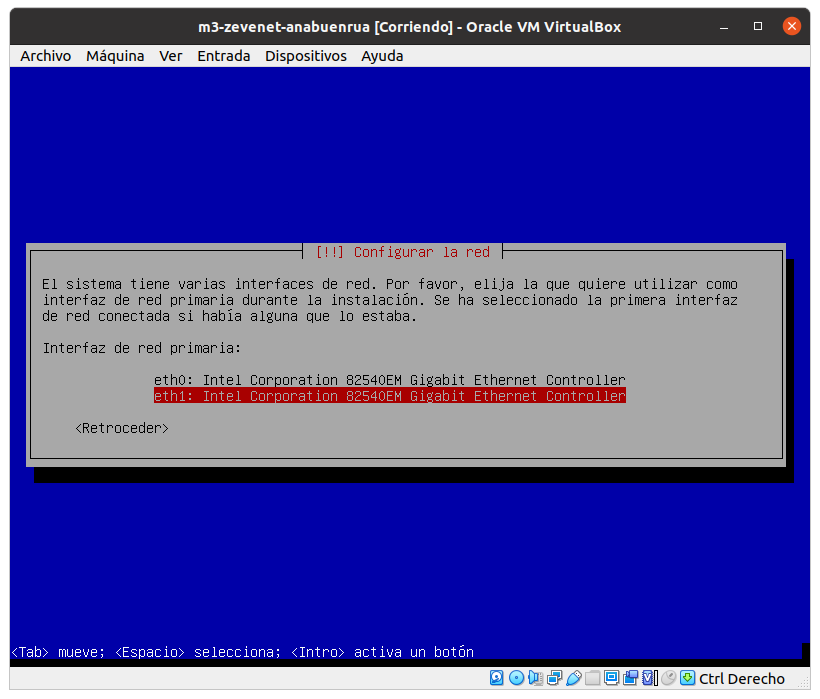
\includegraphics[scale=0.5]{zev_2}
\end{center}
\end{figure}

\begin{figure}[h!]
\begin{center}
\caption{Introducimos la dirección IP durante la instalación de Zevenet}
\label{zev_3}
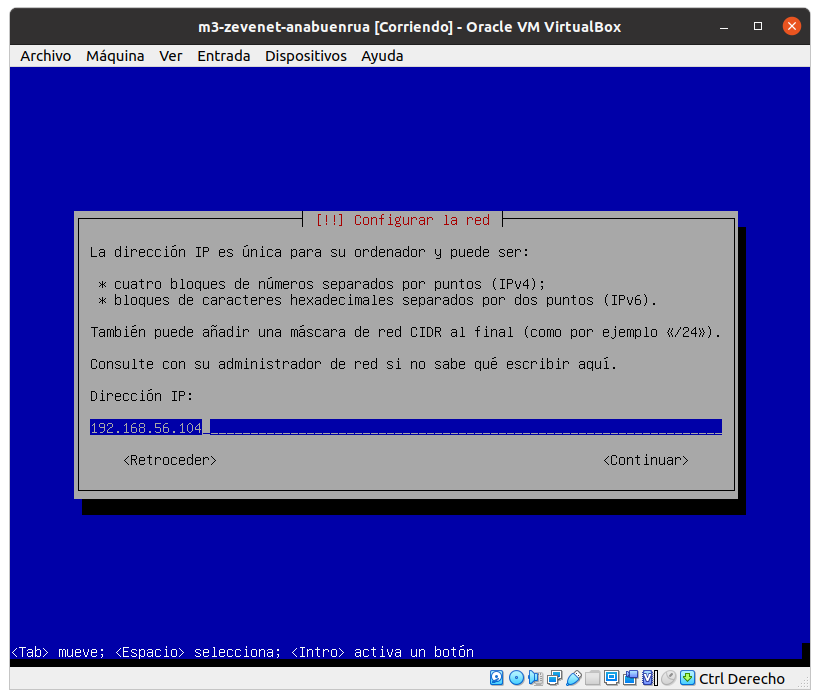
\includegraphics[scale=0.5]{zev_3}
\end{center}
\end{figure}

Dejamos la netmask y gateway por defecto, al igual que el nameserver. Como hostname introduzco mi usuario de la ugr y como contraseña establezco Swap1234.

Seleccionamos la instalación guiada usando todo el disco, dejamos las particiones por defecto y tras instalar el grub completamos la instalación.

Finalmente, iniciamos la máquina, como se ve en \eqref{zev_9}.

\begin{figure}[h!]
\begin{center}
\caption{Zevenet tras la instalación.}
\label{zev_9}
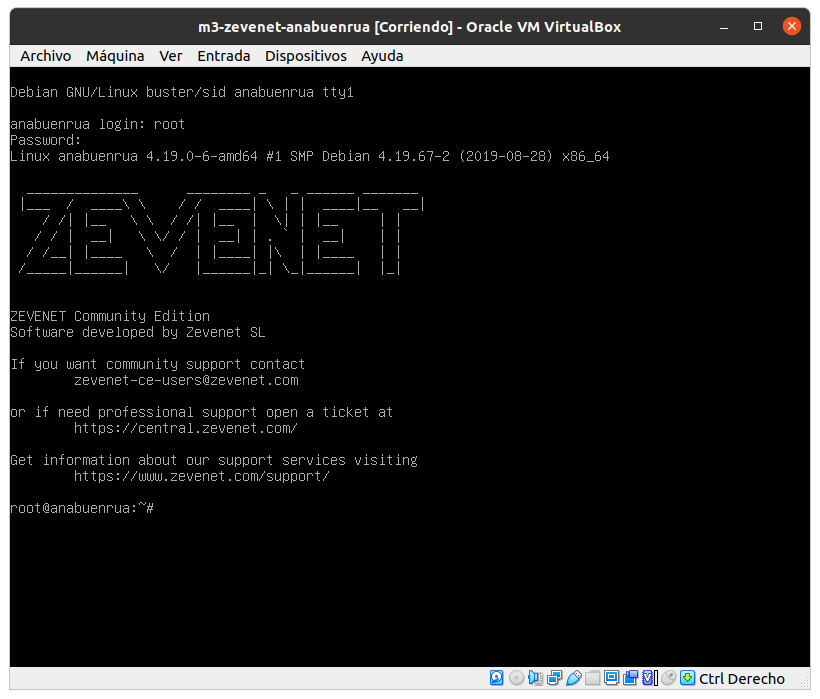
\includegraphics[scale=0.5]{zev_9}
\end{center}
\end{figure}

Accedemos ahora a la dirección 192.168.56.104 por el puerto 444, donde nos identificamos con el usuario y contraseña establecida, como se ve en \eqref{zev_11} y llegamos la dashboard \eqref{zev_12}.

\begin{figure}[h!]
\begin{center}
\caption{Autenticación para acceder al dashboard de Zevenet}
\label{zev_11}
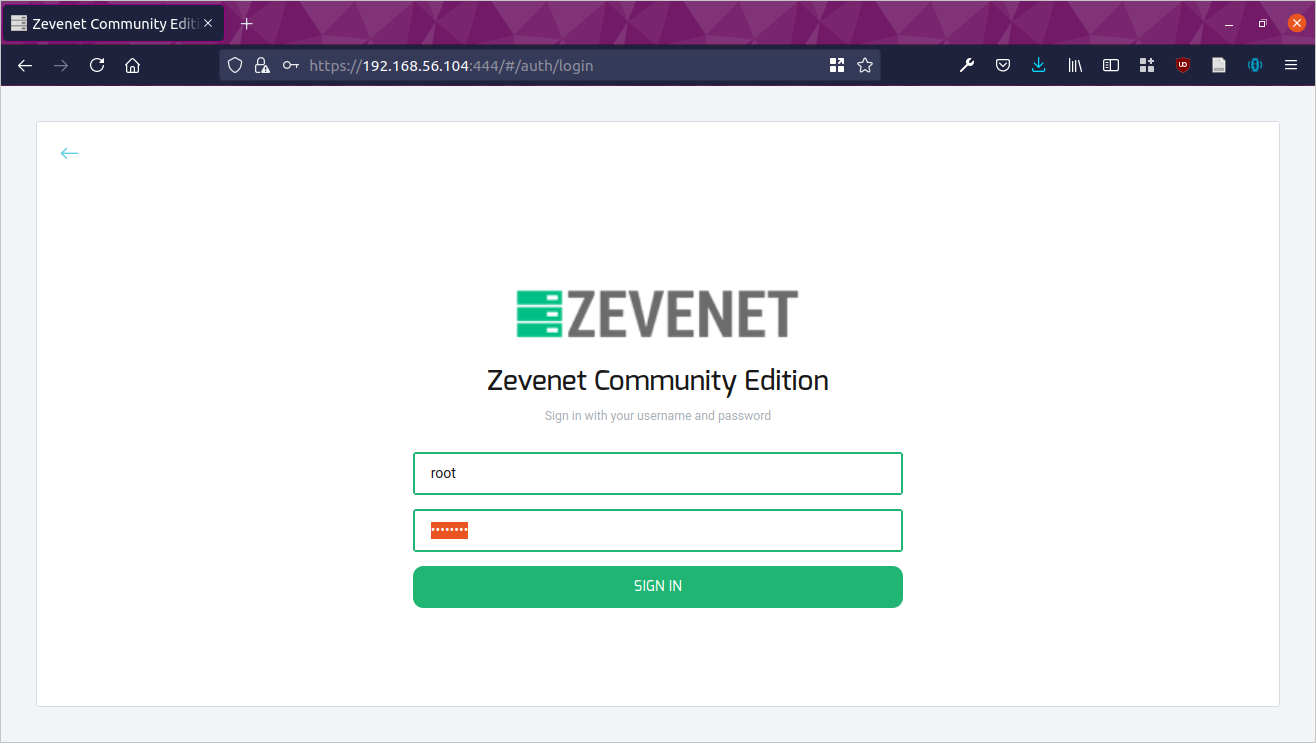
\includegraphics[scale=0.25]{zev_11}
\end{center}
\end{figure}

\begin{figure}[h!]
\begin{center}
\caption{Dashboard de Zevenet}
\label{zev_12}
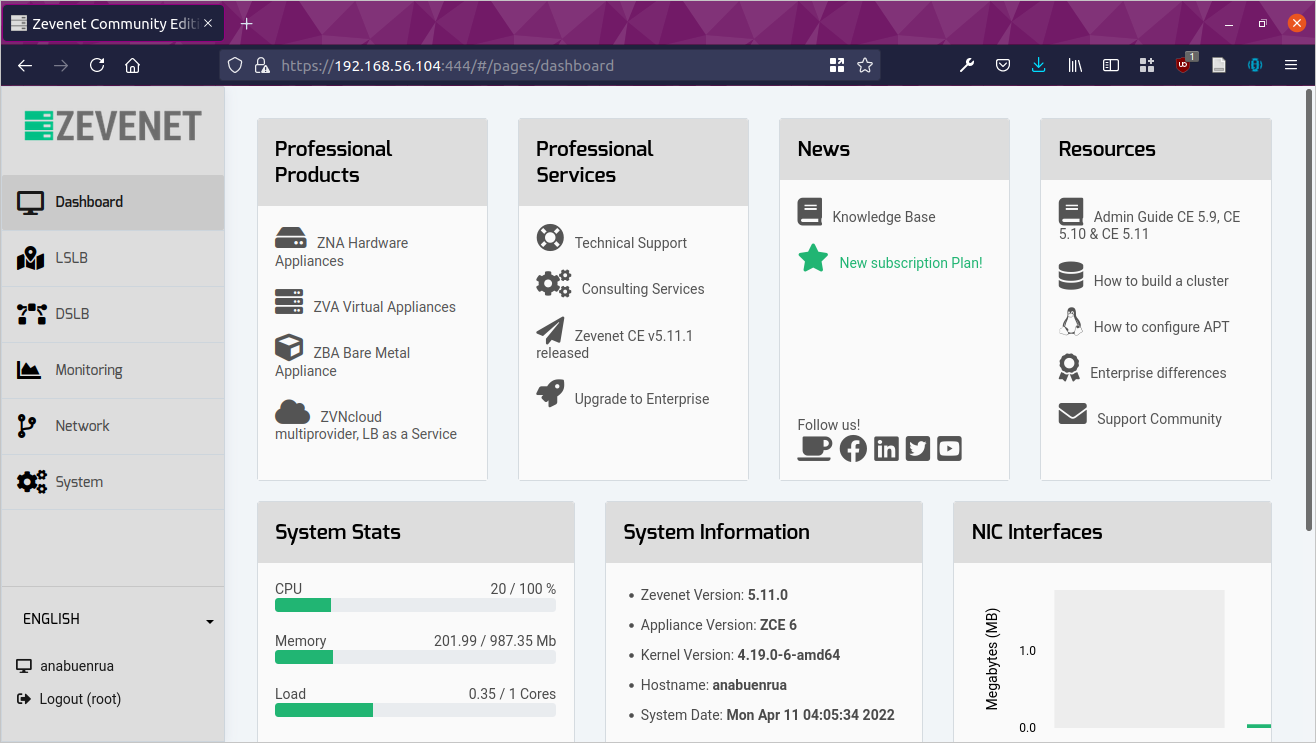
\includegraphics[scale=0.25]{zev_12}
\end{center}
\end{figure}

Ahora, en Network->NIC comprobamos y configuramos las redes para que quede así como en \eqref{zev_13}.

\begin{figure}[h!]
\begin{center}
\caption{Configuración de las redes de Zevenet}
\label{zev_13}
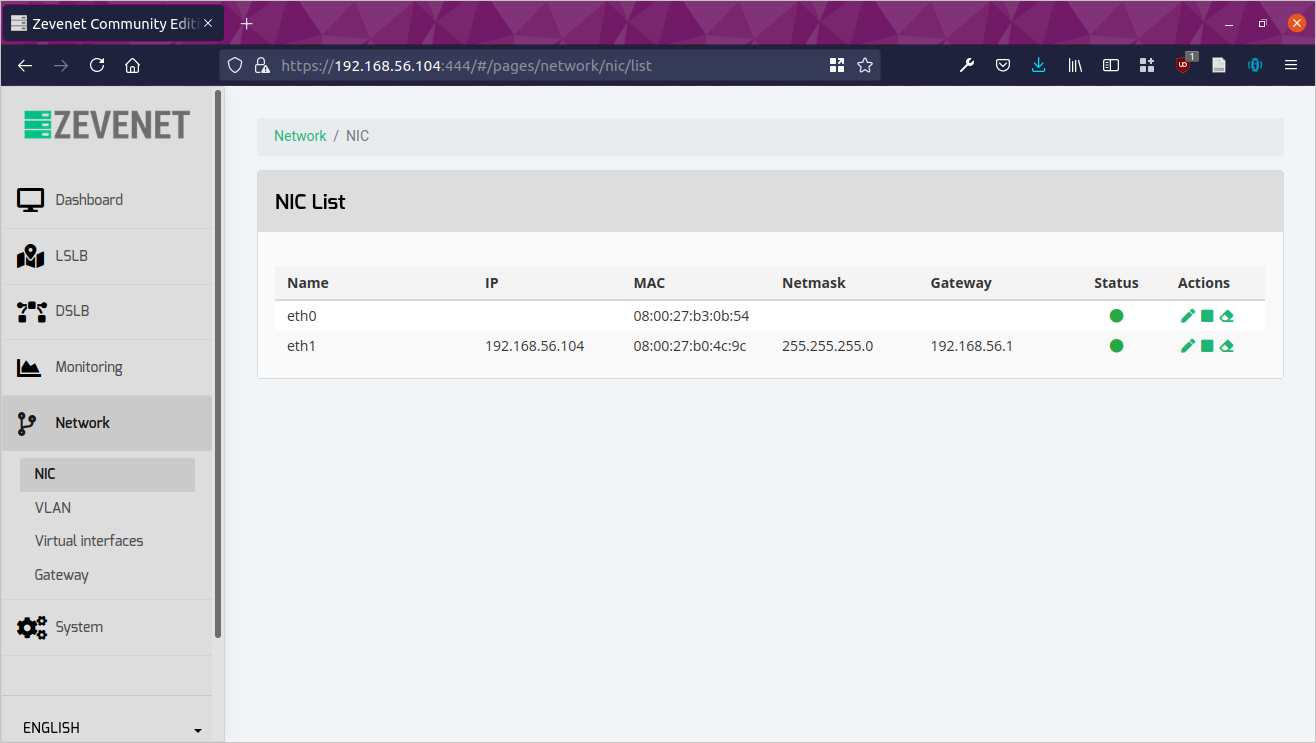
\includegraphics[scale=0.25]{zev_13}
\end{center}
\end{figure}

Y en LSLB-> Farms creamos una nueva granja de red como se ve en \eqref{zev_14}.

\begin{figure}[h!]
\begin{center}
\caption{Creación de una granja en Zevenet}
\label{zev_14}
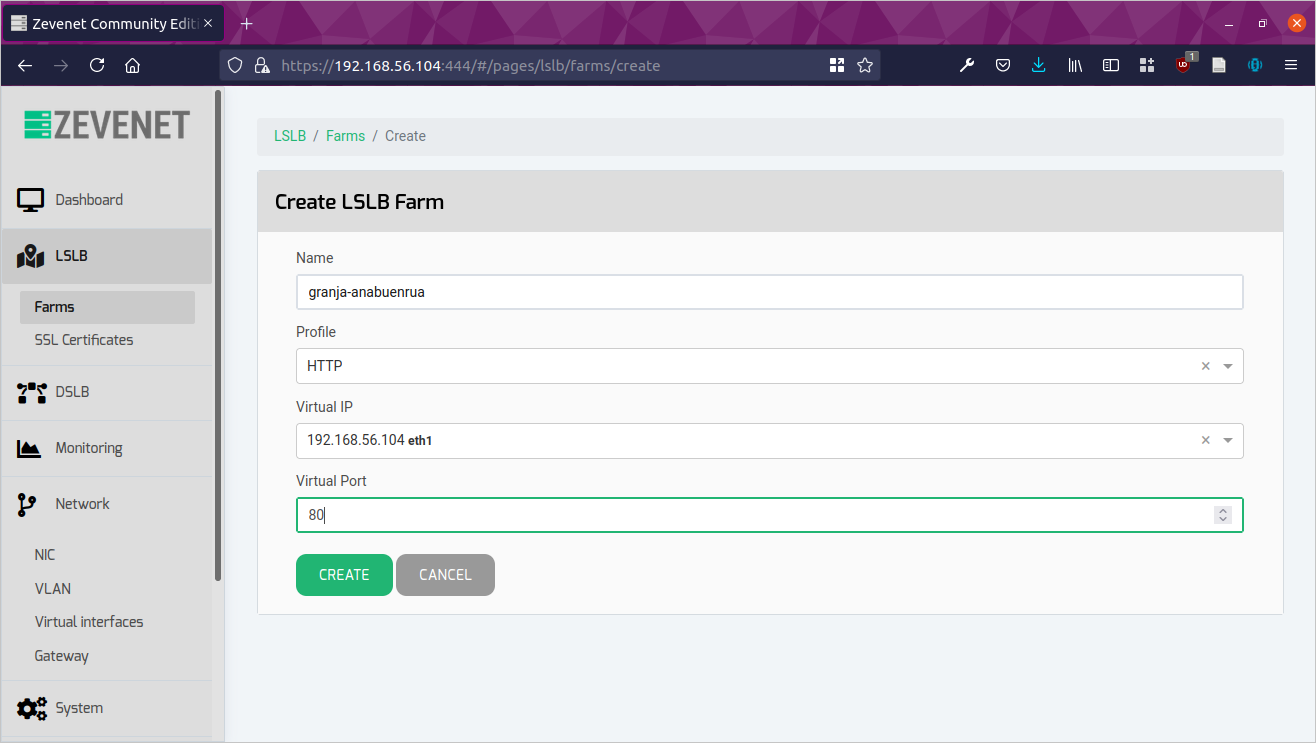
\includegraphics[scale=0.25]{zev_14}
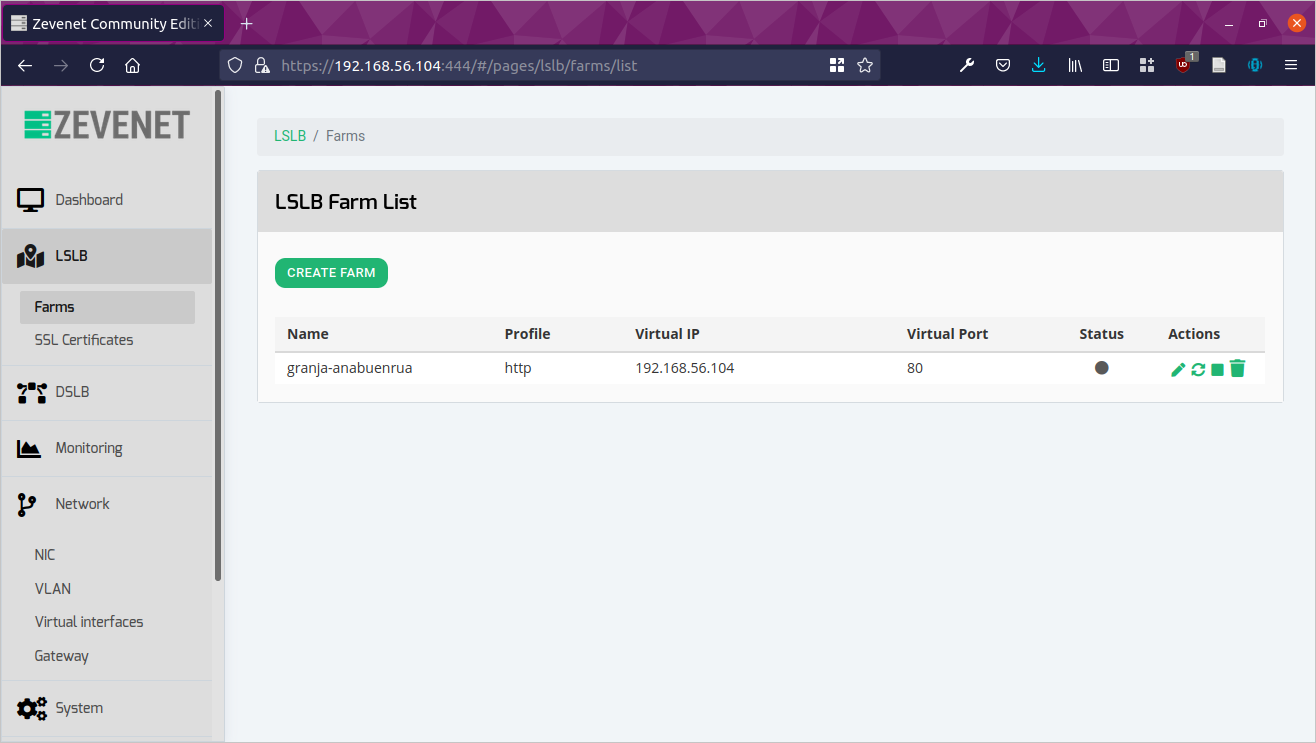
\includegraphics[scale=0.25]{zev_15}
\end{center}
\end{figure}

Ahora, dando a editar podemos ver las opciones avanzadas, puede verse en \eqref{zev_16}. 

\begin{figure}[h!]
\begin{center}
\caption{Opciones avanzadas de una granja en Zevenet}
\label{zev_16}
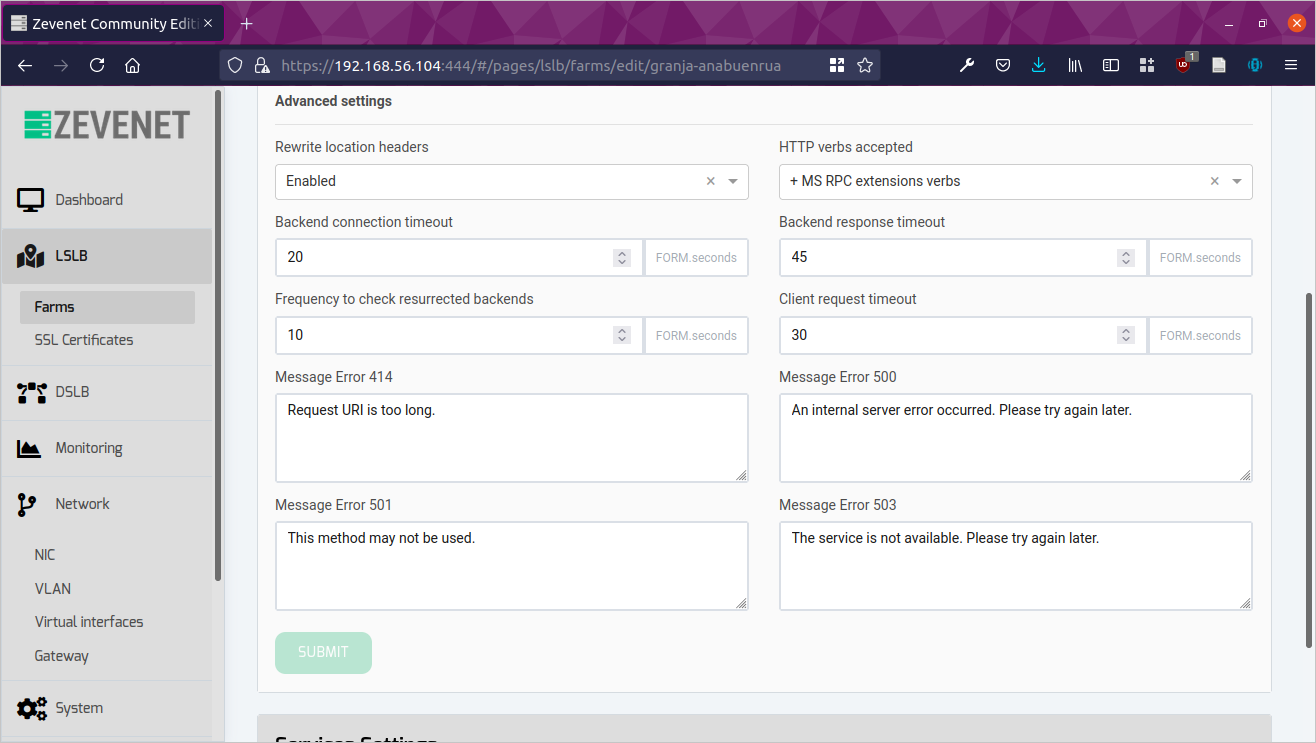
\includegraphics[scale=0.25]{zev_16}
\end{center}
\end{figure}

Y podemos crear un servicio \verb|swap| con m1 y m2 como backends como se muestra en \eqref{zev_17}.

\begin{figure}[h!]
\begin{center}
\caption{Creación del servicio swap en la granja}
\label{zev_17}
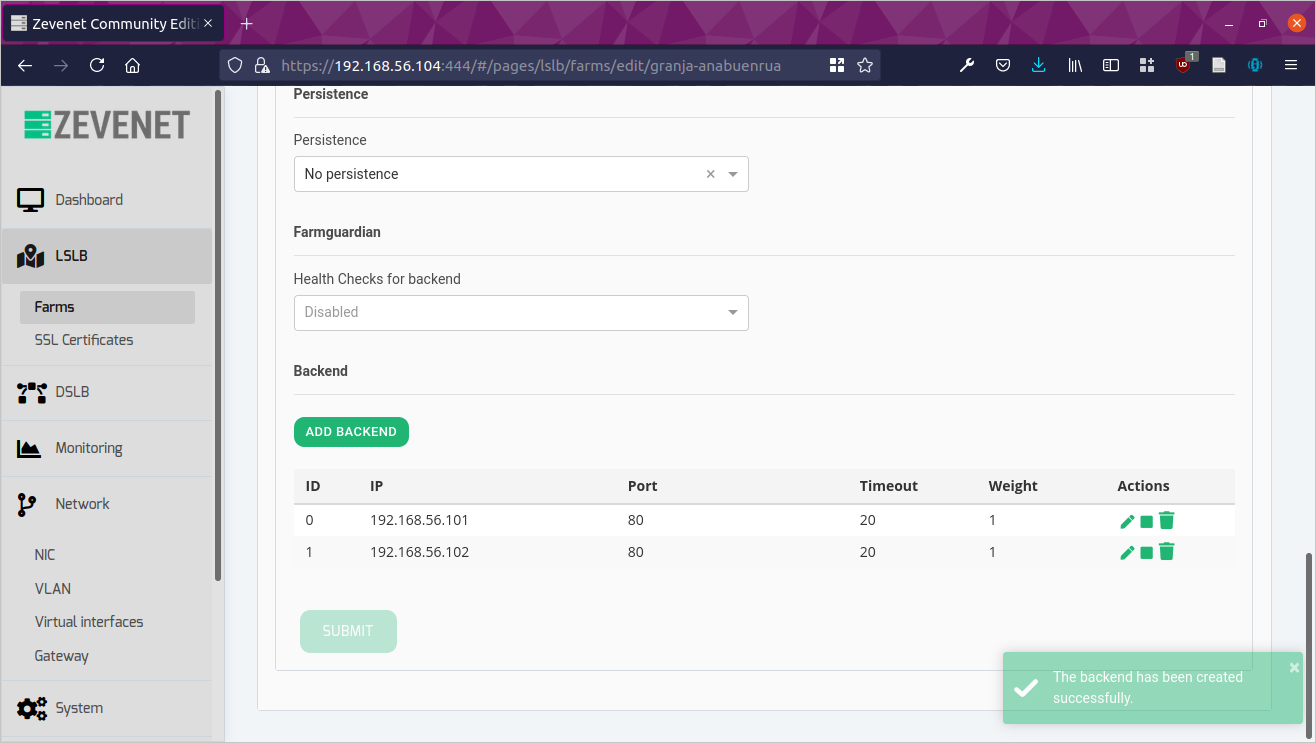
\includegraphics[scale=0.25]{zev_17}
\end{center}
\end{figure}

\section{Opciones avanzadas}

Como opciones avanzadas podemos configurar el timeout de los backend de forma independiente, como ya hemos visto, así como asignar pesos, como se ve en \eqref{zev_19}.

\begin{figure}[h!]
\begin{center}
\caption{Configuración del timeout y asignación de pesos a m1 y m2 en Zevenet.}
\label{zev_19}
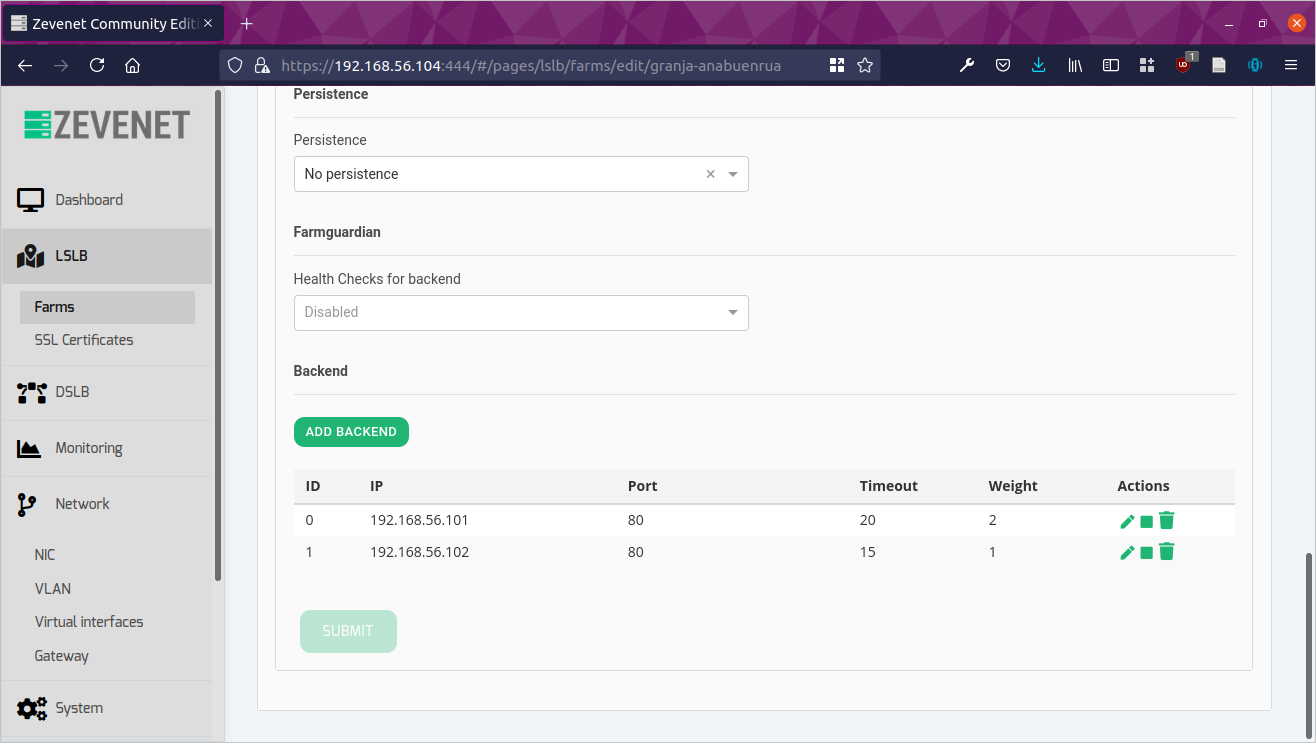
\includegraphics[scale=0.25]{zev_19}
\end{center}
\end{figure}

Al hacer los cambios le damos al botón de restart de la granja y comprobamos que ya funciona.

También se puede configurar la persistencia por sesiones durante un tiempo máximo y comprobaciones del estado de los backend, como se muestra en \eqref{zev_20}.

\begin{figure}[h!]
\begin{center}
\caption{Configuración persistencia de sesiones y comprobaciones del estado de los backend en Zevenet.}
\label{zev_20}
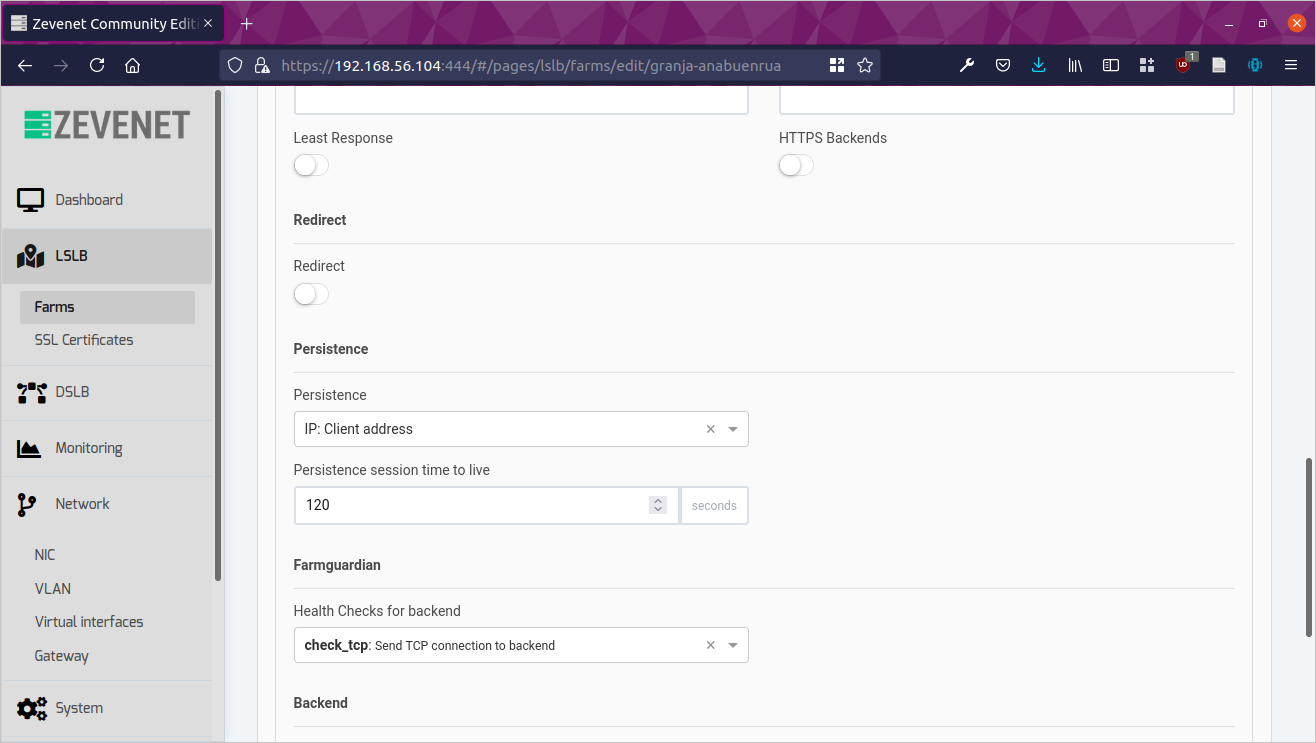
\includegraphics[scale=0.25]{zev_20}
\end{center}
\end{figure}

\chapter{Pound}

Tras asegurarnos de que ninguno de los otros softwares usados está en marcha, descargamos pound, para ello vamos a ejecutar:

\begin{verbatim}
sudo apt-get update
sudo apt-get install pound
\end{verbatim}

Y comprobamos que está funcionando con \verb|sudo systemctl status pound|.

Vamos a editar el fichero de configuración \verb|/etc/pound/pound.cfg| para que quede como en \eqref{pound_2}.

\begin{figure}[h!]
\begin{center}
\caption{Fichero de configuración /etc/pound/pound.cfg .}
\label{pound_2}
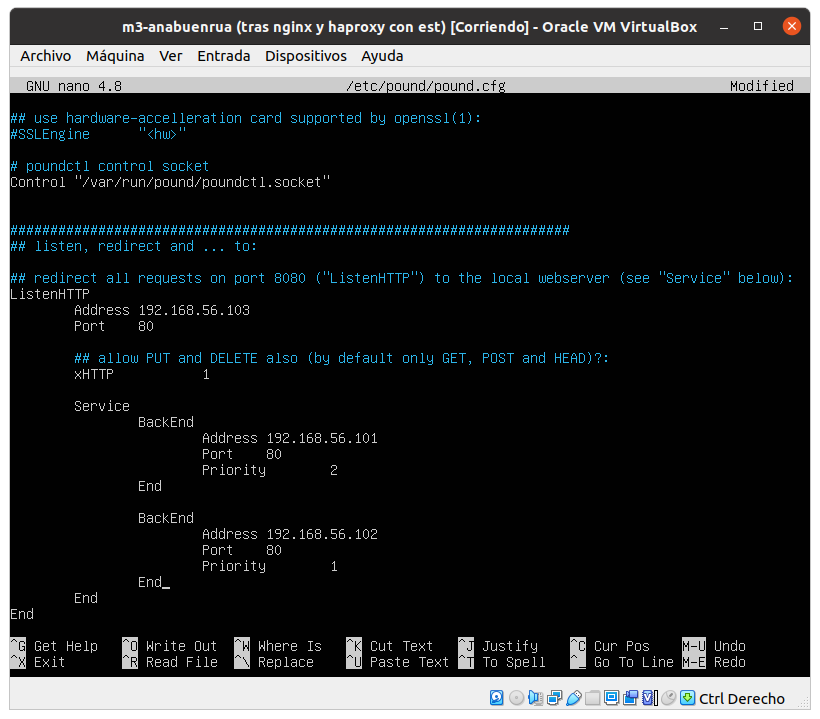
\includegraphics[scale=0.5]{pound_2}
\end{center}
\end{figure}

Y relanzamos el servicio con \verb|sudo systemctl restart pound| y probamos a lanzarlo, pero no funciona, comprobamos el estado con \verb|sudo systemctl status pound| y nos sale un mensaje diciendo que configuremos \verb|startup=1| en \verb|/etc/default/pound|, como se ve en \eqref{pound_3}.

\begin{figure}[h!]
\begin{center}
\caption{Resultado de comprobar el estado de pound con systemctl status}
\label{pound_3}
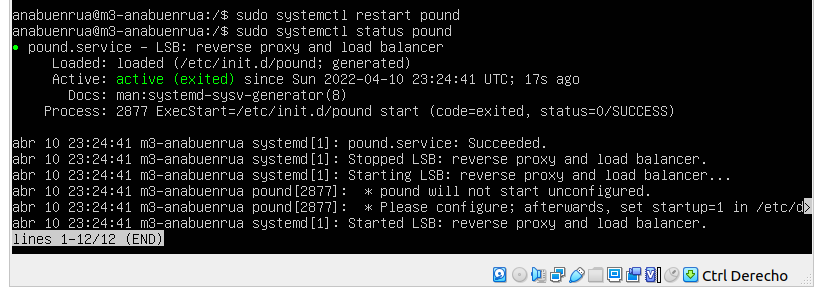
\includegraphics[scale=0.5]{pound_3}
\end{center}
\end{figure}

Editamos \verb|/etc/default/pound| dejándolo como en \eqref{pound_4}.

\begin{figure}[h!]
\begin{center}
\caption{Fichero /etc/default/pound .}
\label{pound_4}
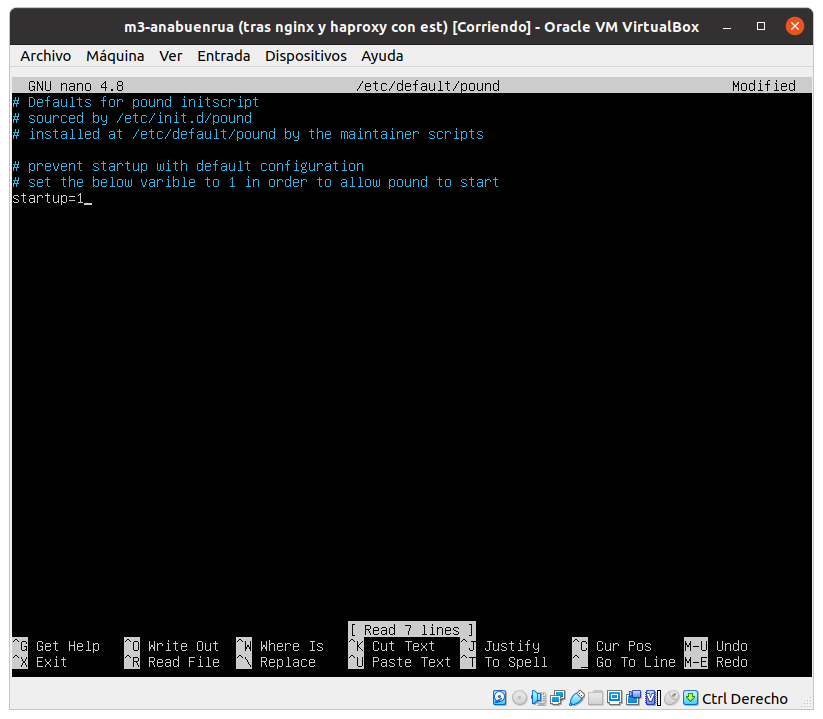
\includegraphics[scale=0.5]{pound_4}
\end{center}
\end{figure}

Tras esto relanzamos el servicio y comprobamos que ahora sí funciona, y al haber establecido las prioridades con m1 el doble de m2, tenemos que m1 recibe el doble de peticiones que m2.

\section{Opciones avanzadas}

Podemos añadir, por ejemplo, a las directivas globales \verb|TimeOut|, que es el tiempo que se espera una respuesta del backend.

xHTTP define los verbos HTTP que se aceptan.

Además, si usamos Emergency, el servidor solo se usará cuando el resto de servidores fallen.

Editamos el fichero de configuración con estas opciones, como se ve en \eqref{pound_5}.

\begin{figure}[h!]
\begin{center}
\caption{Fichero /etc/pound/pound.cfg con opciones avanzadas (emergency).}
\label{pound_5}
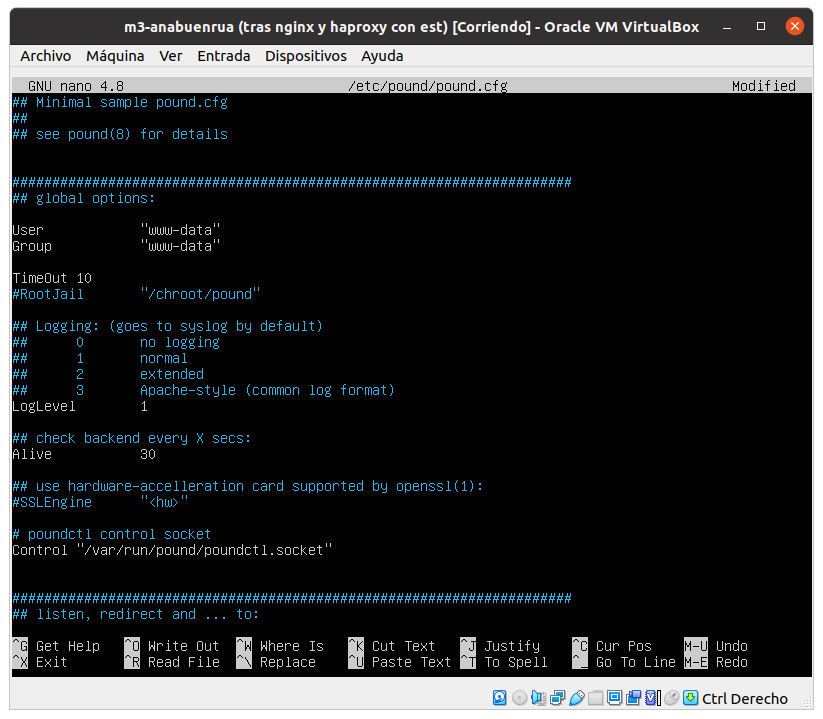
\includegraphics[scale=0.5]{pound_5}
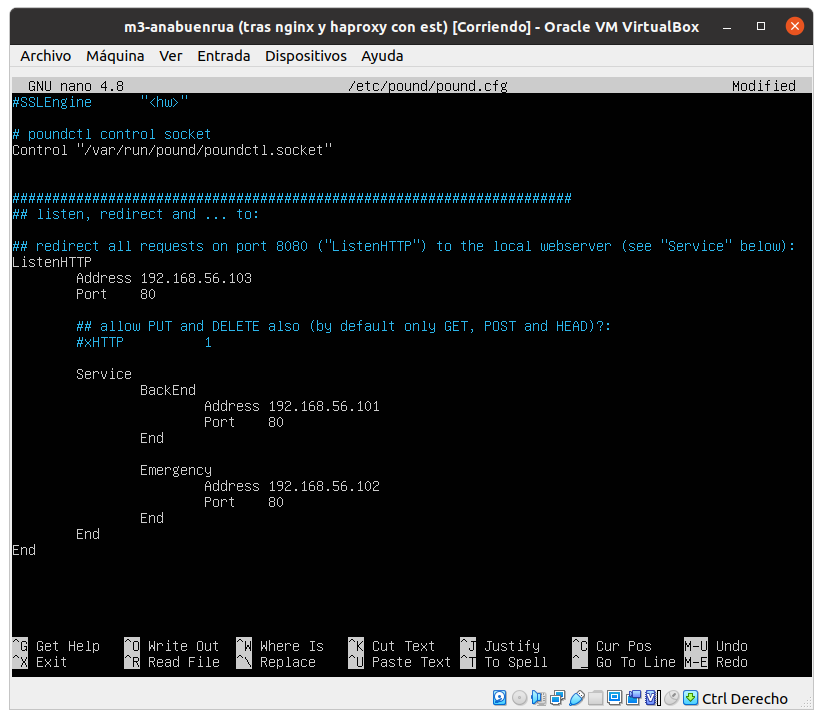
\includegraphics[scale=0.5]{pound_6}
\end{center}
\end{figure}

Relanzamos el servicio y vemos que ahora solo nos atiende m1.

Además, al igual que en los otros sistemas hay algo similar a la ip hash, para que las peticiones de la misma ip las atienda la misma máquina en un margen de tiempo. Esto puede verse en \eqref{pound_7}.

\begin{figure}[h!]
\begin{center}
\caption{Fichero /etc/pound/pound.cfg con opciones avanzadas (session).}
\label{pound_7}
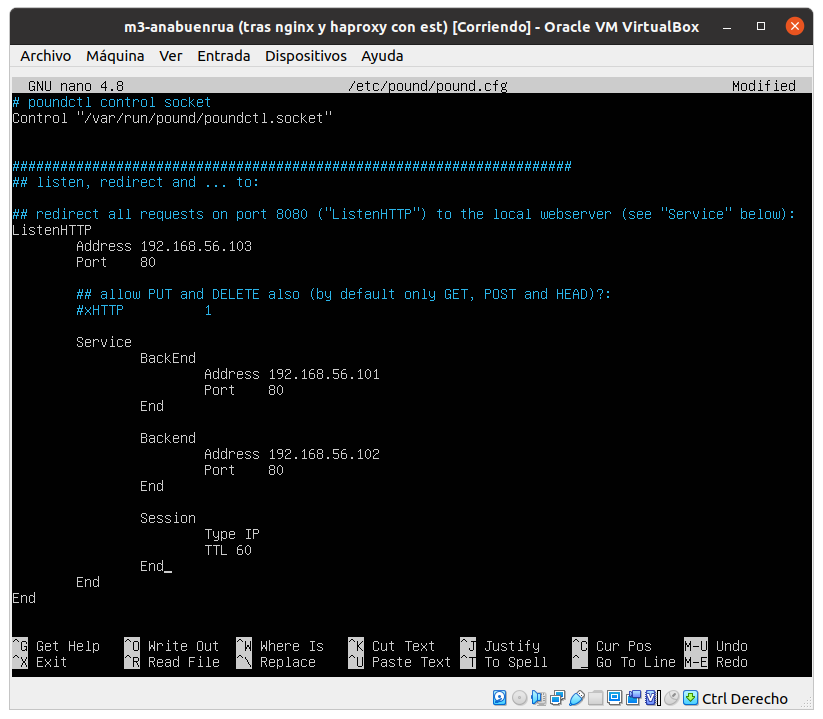
\includegraphics[scale=0.5]{pound_7}
\end{center}
\end{figure}

Y relanzando comprobamos que siempre nos atiende la misma máquina.

Finalmente, y como con nginx y haproxy, se desactiva que se lance al inicio para evitar problemas por usar todos los servicios el mismo puerto con \verb|sudo systemctl disable pound|.

\chapter{Someter la granja web a una carga}

Comenzamos instalando apache benchmark en la máquina anfitriona con el comando:

\begin{verbatim}
sudo apt-get install -y apache2-utils
\end{verbatim}

Ahora, lanzamos nginx y lo configuramos con roundrobin, como antes.

Lanzamos el benchmark, con 10000 peticiones con concurrencia 10:

\begin{verbatim}
ab -n 10000 -c 10 http://192.168.56.103/index.html
\end{verbatim}

Obtenemos la siguiente información, que puede verse en \eqref{bench_2}.

\begin{figure}[h!]
\begin{center}
\caption{Resultado de someter a carga a una granja web con nginx con 10000 peticiones y 10 de concurrencia.}
\label{bench_2}
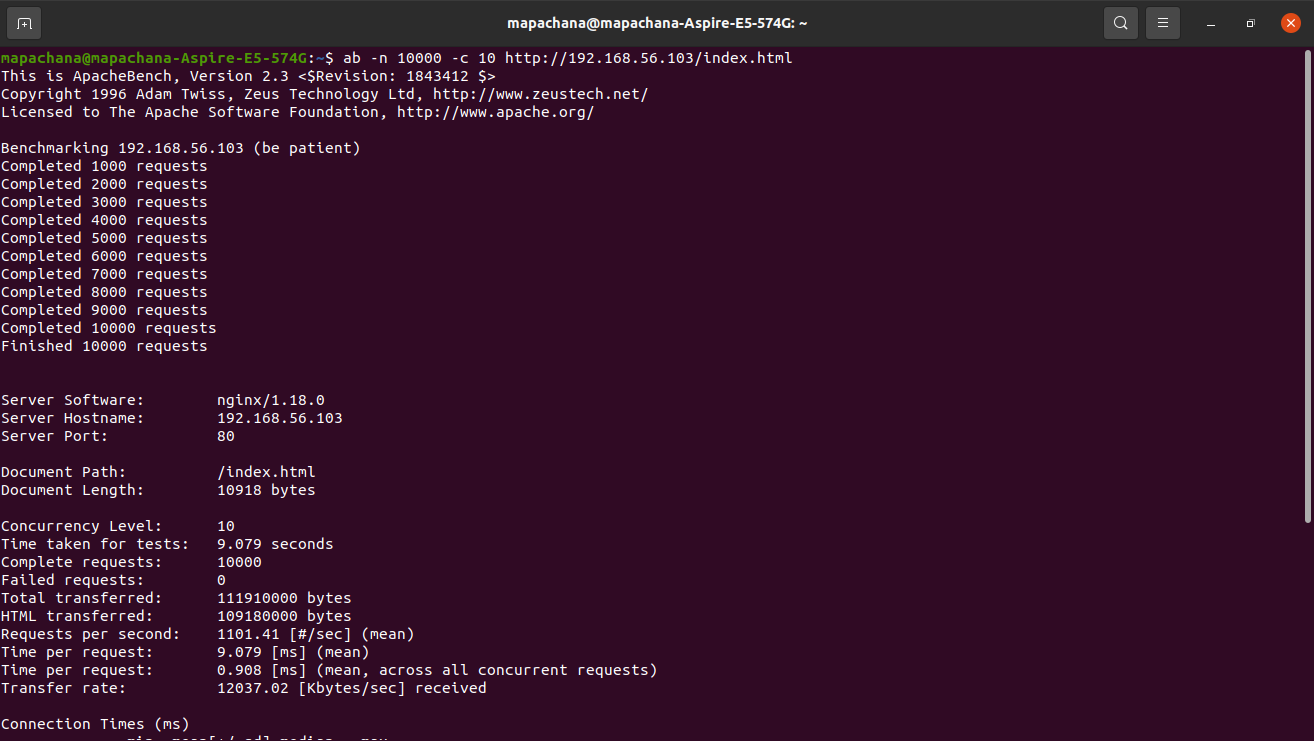
\includegraphics[scale=0.35]{bench_2}
\includegraphics[scale=0.5]{bench_3}
\end{center}
\end{figure}

Donde lo mas relevante son las peticiones por segundo, que es el criterio principal que vamos a usar para comparar.

También llama la atención cuál ha sido el tiempo más largo para atender a una petición.

\section{Otros parámetros}

Otras opciones aparte de \verb|-n| y \verb|-c| para indicar el número de peticiones y la concurrencia son:
\begin{itemize}
\item \verb|-q|: no muestra los mensajes de progreso.
\item \verb|-v|: modo verboso.
\item \verb|-e file.csv|: escribe el tiempo que se tardó en atender cierto porcentaje de las peticiones en el fichero indicado.
\item \verb|-t|: indica el tiempo máximo que va a ejecutarse el benchmark.
\item \verb|-p| y \verb|-u|: indican si la petición es POST o PUT respectivamente, deben usarse con \verb|-T|, que indica la cabecera del content-type.
\end{itemize}

\chapter{Análisis comparativo de distintos balanceadores en base a la carga con AB}

Ahora, se someterá a la misma carga de 10000 peticiones con 10 de concurrencia a todos los balanceadores configurados, cada uno con round robin y ponderación, con m1 atendiendo el doble de peticiones que m2. Los resultados se muestran en la tabla \eqref{tabla}.

\begin{table}[!ht]
\caption{Resultados de someter a carga a las granjas con distintos balanceadores y configuraciones de round robin y ponderación}
    \centering
    \begin{tabular}{|l|l|l|l|}
    \hline
        Balanceador & Modo & Peticiones/s & Longest request (ms) \\ \hline
        nginx & round-robin & 1101.41 & 29 \\ \hline
        nginx & ponderación & 1035.80 & 46 \\ \hline
        haproxy & round-robin & 1018.19 & 31 \\ \hline
        haproxy & ponderación & 1001.13 & 42 \\ \hline
        gobetween & round-robin & 853.46 & 39 \\ \hline
        gobetween & ponderación & 857.36 & 44 \\ \hline
        zevenet & round-robin & 933.23 & 42 \\ \hline
        zevenet & ponderación & 967.92 & 51 \\ \hline
        pound & round-robin & 742.90 & 132 \\ \hline
        pound & ponderación & 733.41 & 121 \\ \hline
    \end{tabular}
\label{tabla}
\end{table}

Para hacer su comprensión más fácil e intuitiva, se han representado estos datos en una gráfica para las peticiones/s \eqref{graf_pet} y otra para las peticiones que más tiempo han llevado \eqref{graf_tiem}.

\begin{figure}[h!]
\begin{center}
\caption{Comparación de peticiones/s respecto a configuraciones de roundrobin y ponderación en cada balanceador}
\label{graf_pet}
\includegraphics[scale=0.05]{peticioness}
\end{center}
\end{figure}

Se aprecia claramente como nginx cosigue mejores prestaciones en roundrobin y ponderación que el resto de balanceadores, siendo así la mejor opción en principio.

En segunda posición, se encontraría haproxy, seguido de zevenet y después gobetween.

Asimismo, destaca como pound consigue las peores en ambas configuraciones, convirtiéndose en la opción menos recomendable a escoger.

\begin{figure}[h!]
\begin{center}
\caption{Comparación de mayor tiempo de respuesta respecto a configuraciones de roundrobin y ponderación en cada balanceador}
\label{graf_tiem}
\includegraphics[scale=0.05]{longest}
\end{center}
\end{figure}

Observando los tiempos de respuesta de las peticiones que más han tardado en atenderse, observamos una tendencia similar a la ya mencionada según las peticiones/s. El mejor sería nginx, seguido de haproxy, luego gobetween, zevenet y finalmente, por mucha distancia con el resto, pound.

Llama la atención como en la configuración por ponderación los tiempos de respuesta son, en general, significativamente mayores a los de round robin, esto puede deberse a que una máquina (m1) recibe el doble de peticiones que la otra, cuando ambas tienen la misma potencia, y por tanto las peticiones que más tardan pueden tardar casi el doble en ser atendidas que en roundrobin.

Pound es el único balanceador para el que los tiempos de respuestas con ponderación son menores a los tiempos de respuesta con roundrobin, lo que puede deberse a una casualidad (habría que lanzar el benchmark más veces y hacer la media) o simplemente ser así el funcionamiento de pound.

Este análisis no es concluyente sobre qué balanceador puede ser mejor para una granja web, pues influyen muchos más factores de los aquí mencionados, pero a juzgar por los datos, el mejor a priori sería nginx y el peor pound.



